\section{\textbf{APPENDIX SNAILSHELL CURVE}} \label{APPENDIX SNAILSHELL CURVE}


\subsection       {Plot of Snailshell curve
	[\ref  {01-img-Plot of Snailshell curve.pdf} ] }
\label{ssec-01-img-Plot of Snailshell curve.pdf}

\subsection       {Snailshell Radius of Curvature
	[\ref      {02-img-Snailshell Radius of Curvature.pdf}] }
\label{ssec-02-img-Snailshell Radius of Curvature.pdf}

\subsection       {Snailshell Validation in LinuxCNC
	[\ref      {03-img-Snailshell-Validation-in-LinuxCNC.png} ] }
\label{ssec-03-img-Snailshell-Validation-in-LinuxCNC.png}

\subsection     {Snailshell Direction of Travel 3D
	[\ref      {04-img-Snailshell Direction of Travel 3D.pdf} ] }
\label{ssec-04-img-Snailshell Direction of Travel 3D.pdf}

\subsection       {Snailshell First and Second Order Taylor's Approx
	[\ref      {05-img-Snailshell-First-and-Second-Order-Taylors-Approx.pdf}] }
\label{ssec-05-img-Snailshell-First-and-Second-Order-Taylors-Approx.pdf}

\subsection       {Snailshell First minus Second Order Taylor's Approx
	[\ref      {06-img-Snailshell-First-minus-Second-Order-Taylors-Approx.pdf}] }
\label{ssec-06-img-Snailshell-First-minus-Second-Order-Taylors-Approx.pdf}

\subsection       {Snailshell Separate First Second Order Taylor's Approx
	[\ref      {07-img-Snailshell-Separation-First-and-Second-Order-Taylors-Approx.pdf} ] }
\label{ssec-07-img-Snailshell-Separation-First-and-Second-Order-Taylors-Approx.pdf}

\subsection       {Snailshell Separation SAL and SCL
	[\ref      {08-img-Snailshell-Separation-SAL-and-SCL.pdf}] }
\label{ssec-08-img-Snailshell-Separation-SAL-and-SCL.pdf}

\subsection       {Snailshell Chord-error in close view 2 scales
	[\ref      {09-img-Snailshell-Chord-error-in-close-view-2-scales.pdf}] }
\label{ssec-09-img-Snailshell-Chord-error-in-close-view-2-scales.pdf}

\subsection       {Snailshell Four Components Feedrate Limit
	[\ref      {10-img-Snailshell-Four-Components-Feedrate-Limit.pdf} ] }
\label{ssec-10-img-Snailshell-Four-Components-Feedrate-Limit.pdf}

\subsection    {Snailshell FrateCommand FrateLimit and Curr-Frate
	[\ref      {11-img-Snailshell-FrateCommand-FrateLimit-and-Curr-Frate.pdf}] }
\label{ssec-11-img-Snailshell-FrateCommand-FrateLimit-and-Curr-Frate.pdf}

\subsection     {Snailshell FeedRateLimit minus CurrFeedRate
	[\ref      {12-img-Snailshell-FeedRateLimit-minus-CurrFeedRate.pdf} ] }
\label{ssec-12-img-Snailshell-FeedRateLimit-minus-CurrFeedRate.pdf}

\subsection     {Snailshell FC20-Nominal X and Y Feedrate Profiles
	[\ref      {13-img-Snailshell-FC20-Nominal-X-and-Y-Feedrate-Profiles.pdf} ] }
\label{ssec-13-img-Snailshell-FC20-Nominal-X-and-Y-Feedrate-Profiles.pdf}

\subsection     {Snailshell FC20 Nominal Tangential Acceleration
	[\ref      {14-img-Snailshell-FC20-Nominal-Tangential-Acceleration.pdf} ] }
\label{ssec-14-img-Snailshell-FC20-Nominal-Tangential-Acceleration.pdf}

\subsection     {Snailshell FC20 Nominal Rising S-Curve Profile
	[\ref      {15-img-Snailshell-FC20-Nominal-Rising-S-Curve-Profile.pdf} ] }
\label{ssec-15-img-Snailshell-FC20-Nominal-Rising-S-Curve-Profile.pdf}

\subsection     {Snailshell FC20 Nominal Falling S-Curve Profile
	[\ref      {16-img-Snailshell-FC20-Nominal-Falling-S-Curve-Profile.pdf}] }
\label{ssec-16-img-Snailshell-FC20-Nominal-Falling-S-Curve-Profile.pdf}

\subsection       {Snailshell FC10 Colored Feedrate Profile data ngcode
	[\ref      {17-img-Snailshell-FC10-Colored-Feedrate-Profile-data_ngcode.png} ] }
\label{ssec-17-img-Snailshell-FC10-Colored-Feedrate-Profile-data_ngcode.png}

\subsection       {Snailshell FC20 Colored Feedrate Profile data ngcode
	[\ref      {18-img-Snailshell-FC20-Colored-Feedrate-Profile-data_ngcode.png} ] }
\label{ssec-18-img-Snailshell-FC20-Colored-Feedrate-Profile-data_ngcode.png}

Continue ...\\

\subsection       {Snailshell FC30 Colored Feedrate Profile data ngcode
	[\ref      {19-img-Snailshell-FC30-Colored-Feedrate-Profile-data_ngcode.png} ] }
\label{ssec-19-img-Snailshell-FC30-Colored-Feedrate-Profile-data_ngcode.png}

\subsection       {Snailshell FC40 Colored Feedrate Profile data ngcode
	[\ref      {20-img-Snailshell-FC40-Colored-Feedrate-Profile-data_ngcode.png} ] }
\label{ssec-20-img-Snailshell-FC40-Colored-Feedrate-Profile-data_ngcode.png}

\subsection       {Snailshell FC10 Tangential Acceleration
	[\ref      {21-img-Snailshell-FC10-Tangential-Acceleration.pdf}] }
\label{ssec-21-img-Snailshell-FC10-Tangential-Acceleration.pdf}

\subsection       {Snailshell FC20 Tangential Acceleration
	[\ref      {22-img-Snailshell-FC20-Tangential-Acceleration.pdf}] }
\label{ssec-22-img-Snailshell-FC20-Tangential-Acceleration.pdf}

\subsection       {Snailshell FC30 Tangential Acceleration
	[\ref      {23-img-Snailshell-FC30-Tangential-Acceleration.pdf}] }
\label{ssec-23-img-Snailshell-FC30-Tangential-Acceleration.pdf}

\subsection       {Snailshell FC40 Tangential Acceleration
	[\ref      {24-img-Snailshell-FC40-Tangential-Acceleration.pdf}] }
\label{ssec-24-img-Snailshell-FC40-Tangential-Acceleration.pdf}

\subsection       {Snailshell FC20 Nominal Separation NAL and NCL
	[\ref      {25-img-Snailshell-FC20-Nominal-Separation-NAL-and-NCL.pdf}] }
\label{ssec-25-img-Snailshell-FC20-Nominal-Separation-NAL-and-NCL.pdf}

\subsection       {Snailshell SAL minus SCL for FC10 FC20 FC30 FC40
	[\ref      {26-img-Snailshell-Difference-SAL-minus-SCL-for-FC10-FC20-FC30-FC40.pdf}] }
\label{ssec-26-img-Snailshell-Difference-SAL-minus-SCL-for-FC10-FC20-FC30-FC40.pdf}


\subsection       {Snailshell FC10 FrateCmd CurrFrate X-Frate Y-Frate
	[\ref      {27-img-Snailshell-FC10-FrateCmd-CurrFrate-X-Frate-Y-Frate.pdf}] }
\label{ssec-27-img-Snailshell-FC10-FrateCmd-CurrFrate-X-Frate-Y-Frate.pdf}

\subsection       {Snailshell FC20 FrateCmd CurrFrate X-Frate Y-Frate
	[\ref      {28-img-Snailshell-FC20-FrateCmd-CurrFrate-X-Frate-Y-Frate.pdf}] }
\label{ssec-28-img-Snailshell-FC20-FrateCmd-CurrFrate-X-Frate-Y-Frate.pdf}

\subsection       {Snailshell FC30 FrateCmd CurrFrate X-Frate Y-Frate
	[\ref      {29-img-Snailshell-FC30-FrateCmd-CurrFrate-X-Frate-Y-Frate.pdf}] }
\label{ssec-29-img-Snailshell-FC30-FrateCmd-CurrFrate-X-Frate-Y-Frate.pdf}

\subsection       {Snailshell FC40 FrateCmd CurrFrate X-Frate Y-Frate
	[\ref      {30-img-Snailshell-FC40-FrateCmd-CurrFrate-X-Frate-Y-Frate.pdf}] }
\label{ssec-30-img-Snailshell-FC40-FrateCmd-CurrFrate-X-Frate-Y-Frate.pdf}

\subsection       {Snailshell FC10 Four Components FeedrateLimit
	[\ref      {31-img-Snailshell-FC10-Four-Components-FeedrateLimit.pdf}] }
\label{ssec-31-img-Snailshell-FC10-Four-Components-FeedrateLimit.pdf}

\subsection       {Snailshell FC20 Four Components FeedrateLimit
	[\ref      {32-img-Snailshell-FC20-Four-Components-FeedrateLimit.pdf}] }
\label{ssec-32-img-Snailshell-FC20-Four-Components-FeedrateLimit.pdf}

\subsection       {Snailshell FC30 Four Components FeedrateLimit
	[\ref      {33-img-Snailshell-FC30-Four-Components-FeedrateLimit.pdf}] }
\label{ssec-33-img-Snailshell-FC30-Four-Components-FeedrateLimit.pdf}

\subsection       {Snailshell FC40 Four Components FeedrateLimit
	[\ref      {34-img-Snailshell-FC40-Four-Components-FeedrateLimit.pdf}]}
\label{ssec-34-img-Snailshell-FC40-Four-Components-FeedrateLimit.pdf}

\subsection       {Snailshell Histogram Points FC10 FC20 FC30 FC40
	[\ref      {35-img-Snailshell-Histogram-Points-FC10-FC20-FC30-FC40.pdf}] }
\label{ssec-35-img-Snailshell-Histogram-Points-FC10-FC20-FC30-FC40.pdf}

\subsection    {Snailshell Table distribution of interpolated points
	[\ref      {tab-Snailshell Table distribution of interpolated points}] }
\label{ssec-tab-Snailshell Table distribution of interpolated points}

\subsection         {Snailshell Table FC10-20-30-40 Run Performance data
	[\ref      {tab-app4-Snailshell-Table-FC10-20-30-40-Run-Performance-data}] }
\label{ssec-tab-app4-Snailshell-Table-FC10-20-30-40-Run-Performance-data}


%% =====================================================
%% =====================================================
\clearpage
\pagebreak

\begin{figure}
	\caption     {Plot of Snailshell curve}
	\label{01-img-Plot of Snailshell curve.pdf}
	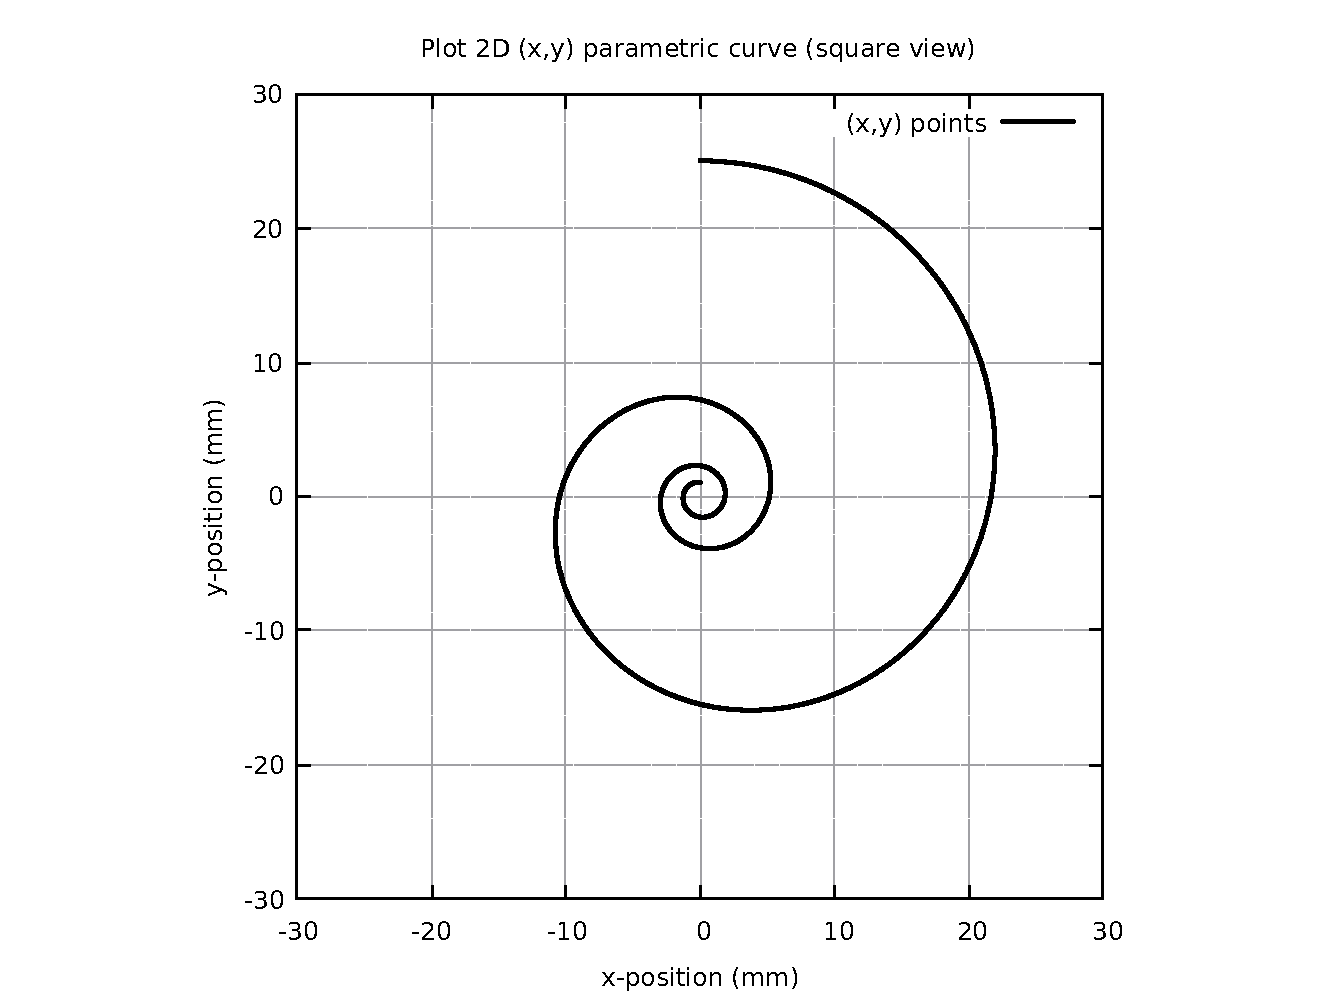
\includegraphics[width=1.00\textwidth]{Chap4/appendix/app-Snailshell/plots/01-img-Plot of Snailshell curve.pdf}
\end{figure}	


\begin{figure}
	\caption     {Snailshell Radius of Curvature}
	\label{02-img-Snailshell Radius of Curvature.pdf}
	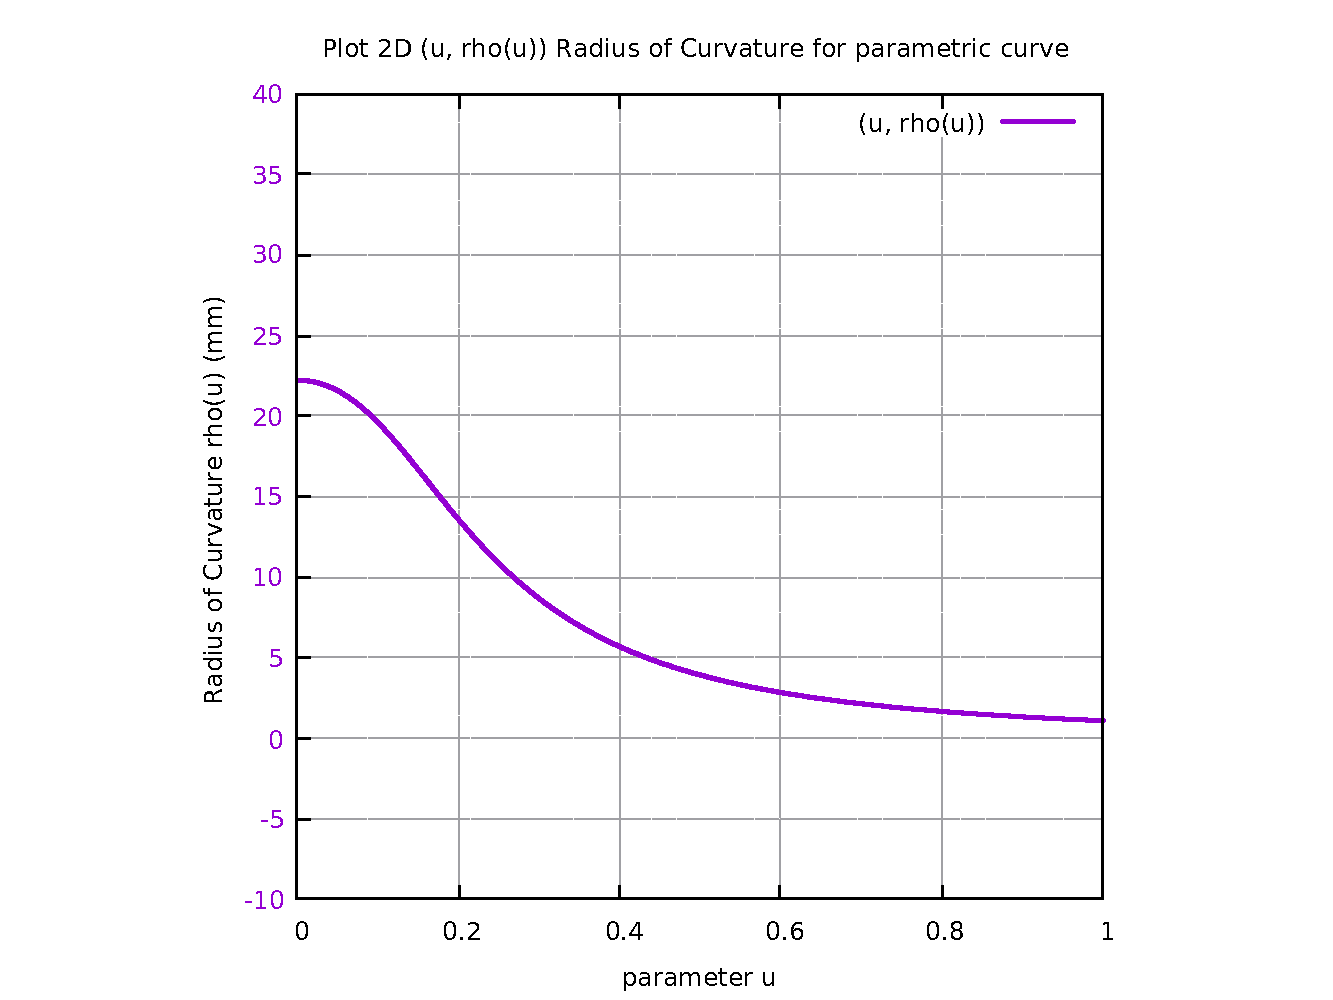
\includegraphics[width=1.00\textwidth]{Chap4/appendix/app-Snailshell/plots/02-img-Snailshell Radius of Curvature.pdf} 
\end{figure}	


%% ==================================================
\clearpage
\pagebreak

\begin{figure}
	\caption     {Snailshell Validation in LinuxCNC}
	\label{03-img-Snailshell-Validation-in-LinuxCNC.png}
	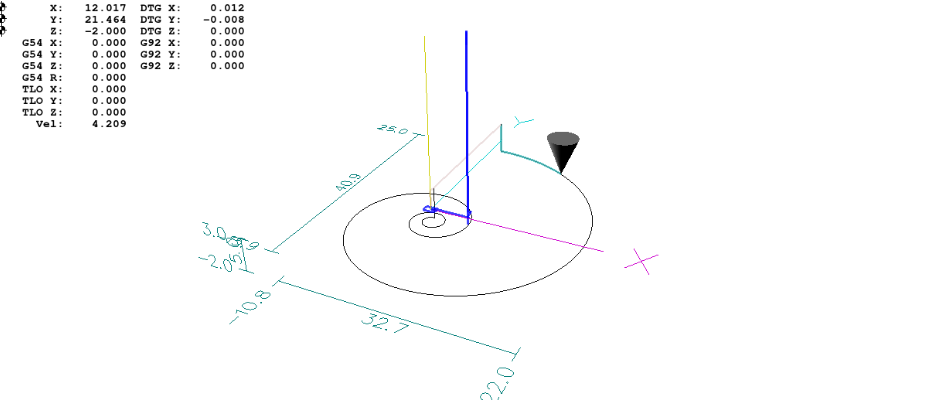
\includegraphics[width=1.00\textwidth]{Chap4/appendix/app-Snailshell/plots/03-img-Snailshell-Validation-in-LinuxCNC.png}
\end{figure}


\begin{figure}
	\caption     {Snailshell Direction of Travel 3D}
	\label{04-img-Snailshell Direction of Travel 3D.pdf}
	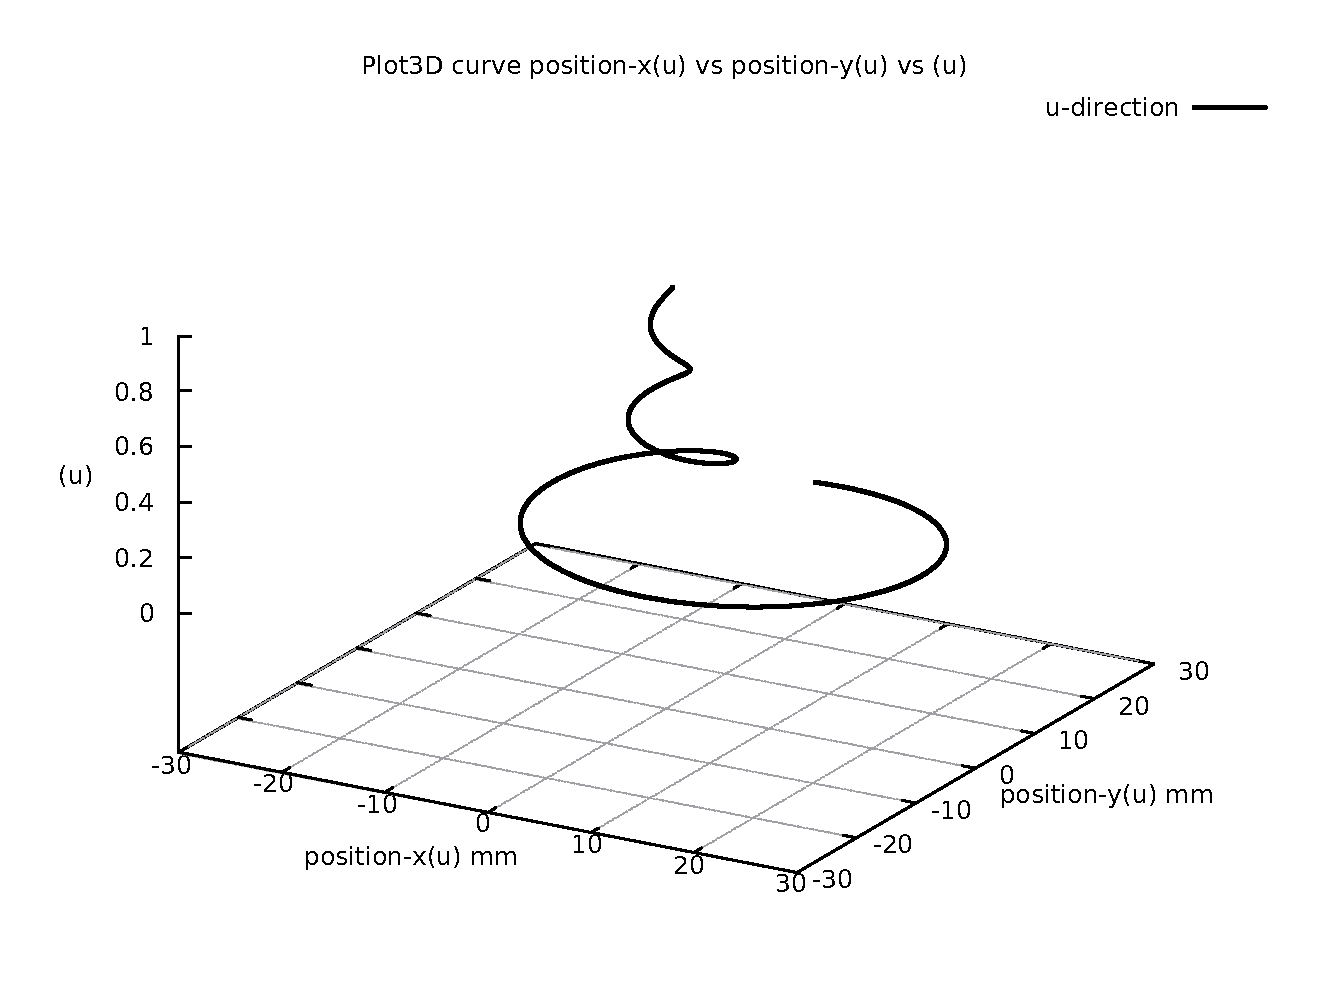
\includegraphics[width=1.00\textwidth]{Chap4/appendix/app-Snailshell/plots/04-img-Snailshell Direction of Travel 3D.pdf}
\end{figure}

%% ==================================================
\clearpage
\pagebreak

\begin{figure}
	\caption     {Snailshell First and Second Order Taylor's Approximation}
	\label{05-img-Snailshell-First-and-Second-Order-Taylors-Approx.pdf}
	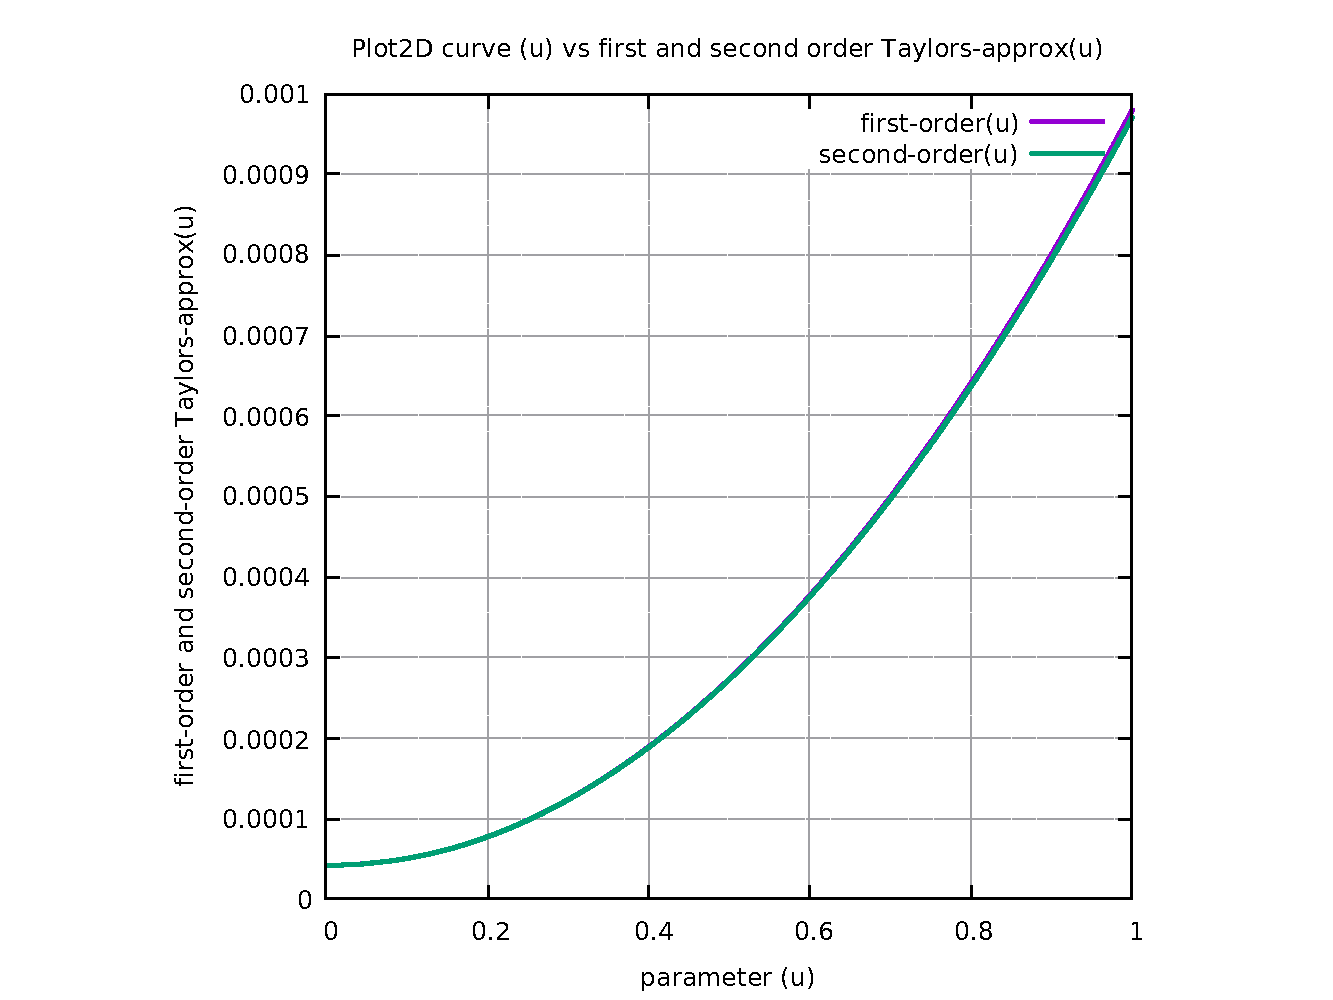
\includegraphics[width=1.00\textwidth]{Chap4/appendix/app-Snailshell/plots/05-img-Snailshell-First-and-Second-Order-Taylors-Approx.pdf}
\end{figure}


\begin{figure}
	\caption     {Snailshell First minus Second Order Taylor's Approximation}
	\label{06-img-Snailshell-First-minus-Second-Order-Taylors-Approx.pdf}
	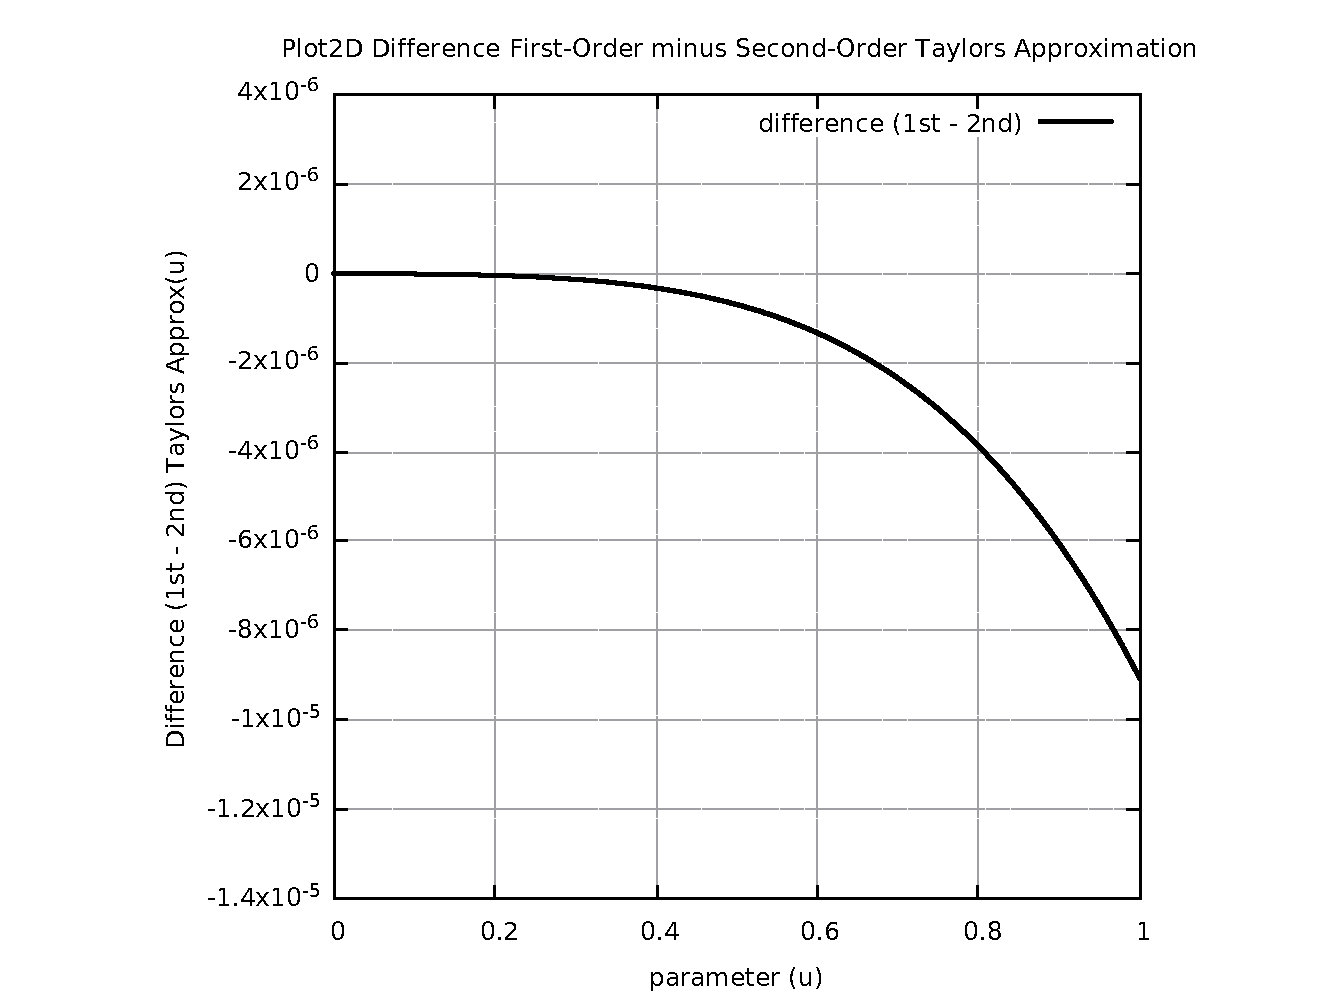
\includegraphics[width=1.00\textwidth]{Chap4/appendix/app-Snailshell/plots/06-img-Snailshell-First-minus-Second-Order-Taylors-Approx.pdf}
\end{figure}

%% ==================================================
\clearpage
\pagebreak

\begin{figure}
	\caption     {Snailshell Separation First and Second Order Taylor's Approximation}
	\label{07-img-Snailshell-Separation-First-and-Second-Order-Taylors-Approx.pdf}
	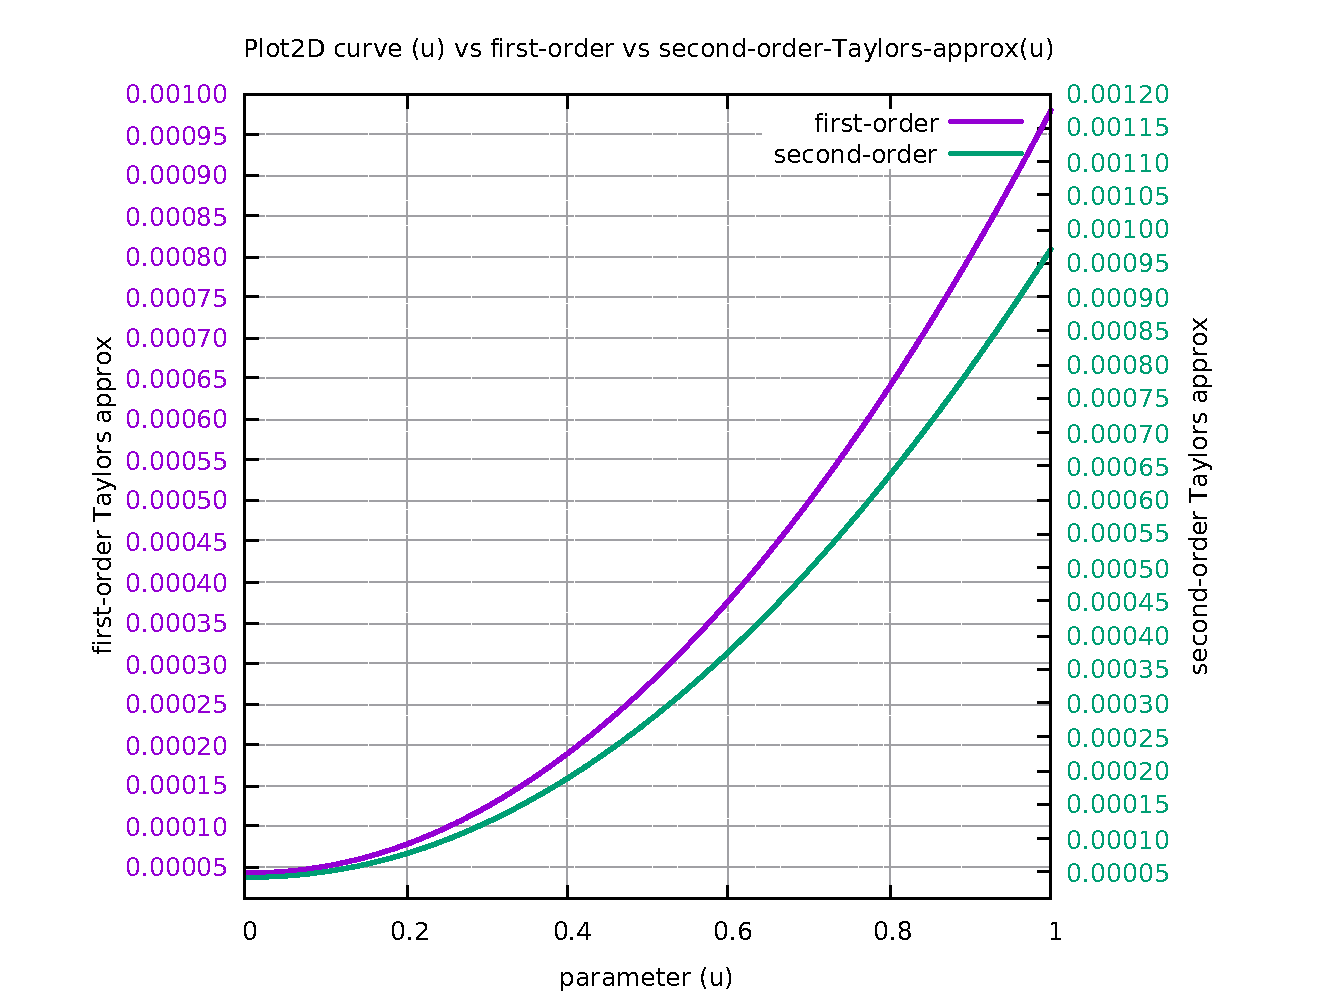
\includegraphics[width=1.00\textwidth]{Chap4/appendix/app-Snailshell/plots/07-img-Snailshell-Separation-First-and-Second-Order-Taylors-Approx.pdf}
\end{figure}


\begin{figure}
	\caption     {Snailshell Separation SAL and SCL}
	\label{08-img-Snailshell-Separation-SAL-and-SCL.pdf}
	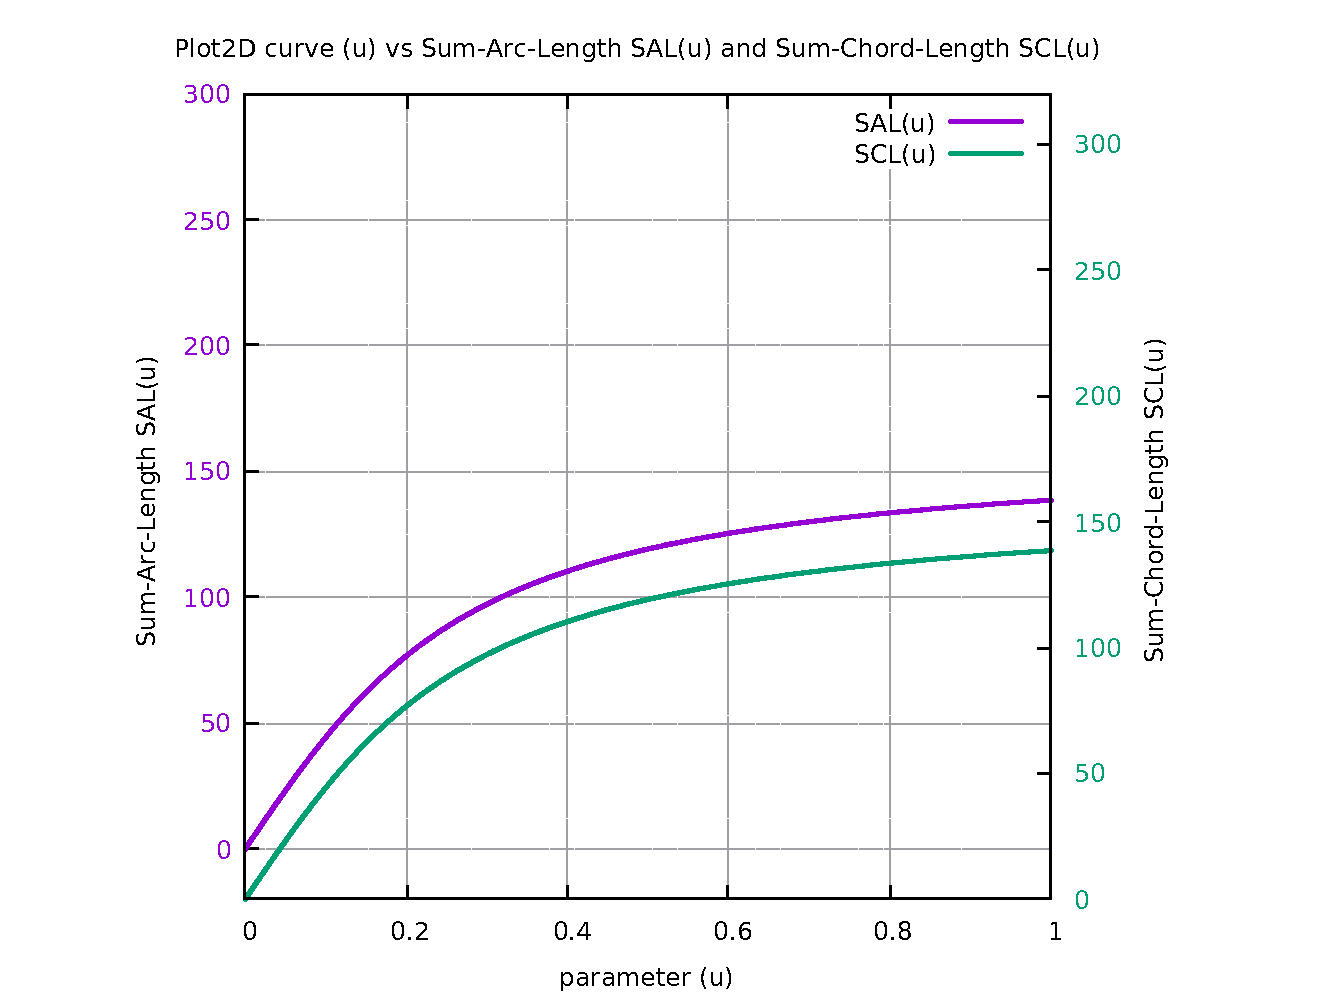
\includegraphics[width=1.00\textwidth]{Chap4/appendix/app-Snailshell/plots/08-img-Snailshell-Separation-SAL-and-SCL.pdf}
\end{figure}

%% ==================================================
\clearpage
\pagebreak

\begin{figure}
	\caption     {Snailshell Chord-error in close view 2 scales}
	\label{09-img-Snailshell-Chord-error-in-close-view-2-scales.pdf}
	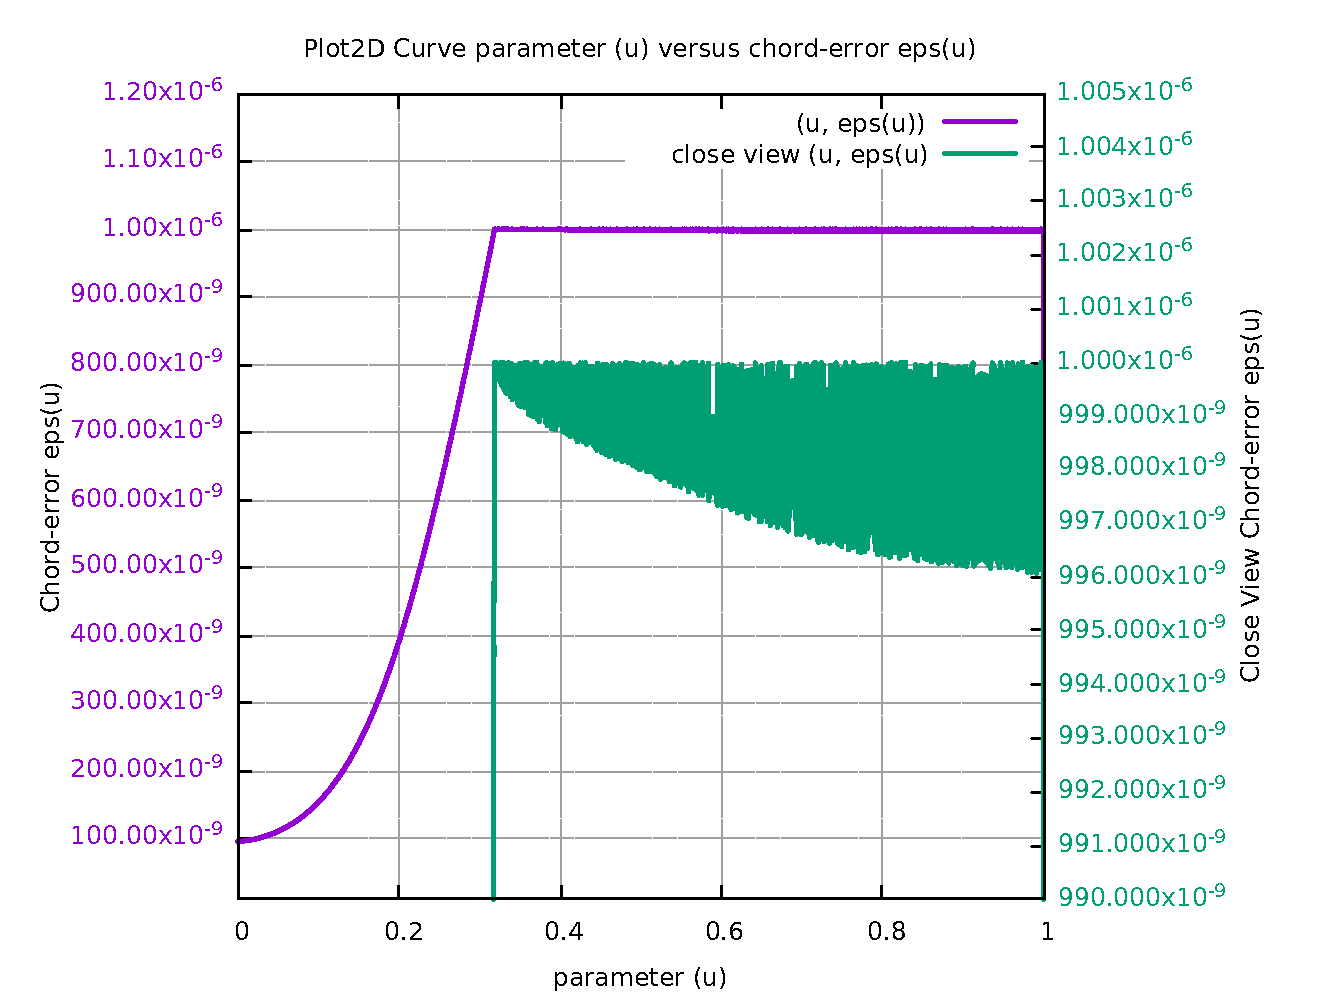
\includegraphics[width=1.00\textwidth]{Chap4/appendix/app-Snailshell/plots/09-img-Snailshell-Chord-error-in-close-view-2-scales.pdf}
\end{figure}

\begin{figure}
	\caption     {Snailshell Four Components Feedrate Limit}
	\label{10-img-Snailshell-Four-Components-Feedrate-Limit.pdf}
	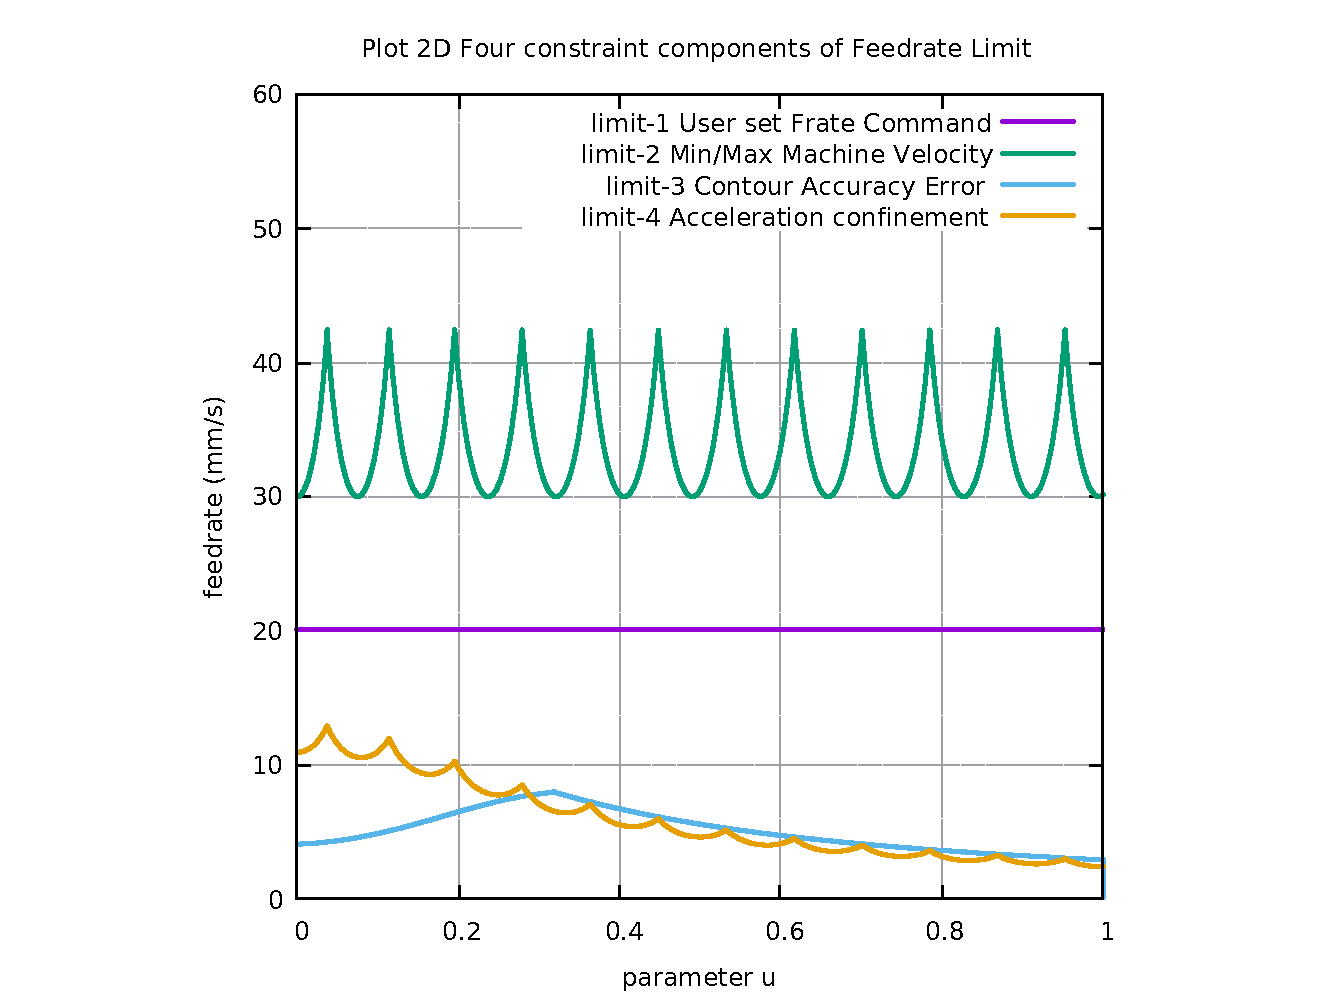
\includegraphics[width=1.00\textwidth]{Chap4/appendix/app-Snailshell/plots/10-img-Snailshell-Four-Components-Feedrate-Limit.pdf}
\end{figure}

%% ==================================================
\clearpage
\pagebreak

\begin{figure}
	\caption     {Snailshell FrateCommand FrateLimit and Curr-Frate}
	\label{11-img-Snailshell-FrateCommand-FrateLimit-and-Curr-Frate.pdf}
	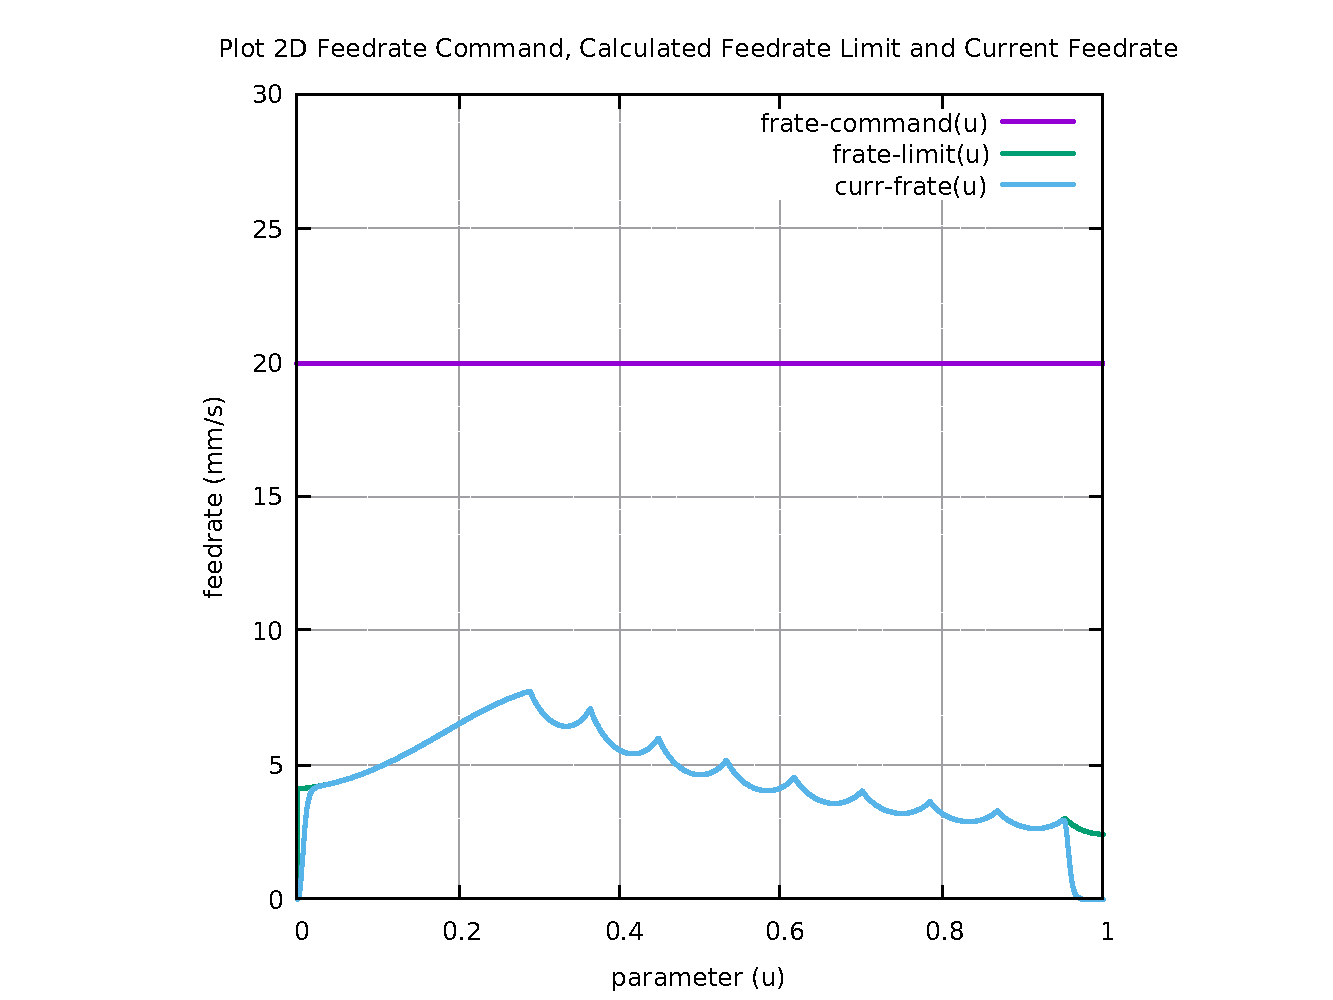
\includegraphics[width=1.00\textwidth]{Chap4/appendix/app-Snailshell/plots/11-img-Snailshell-FrateCommand-FrateLimit-and-Curr-Frate.pdf}
\end{figure}

\begin{figure}
	\caption     {Snailshell FeedRateLimit minus CurrFeedRate}
	\label{12-img-Snailshell-FeedRateLimit-minus-CurrFeedRate.pdf}
	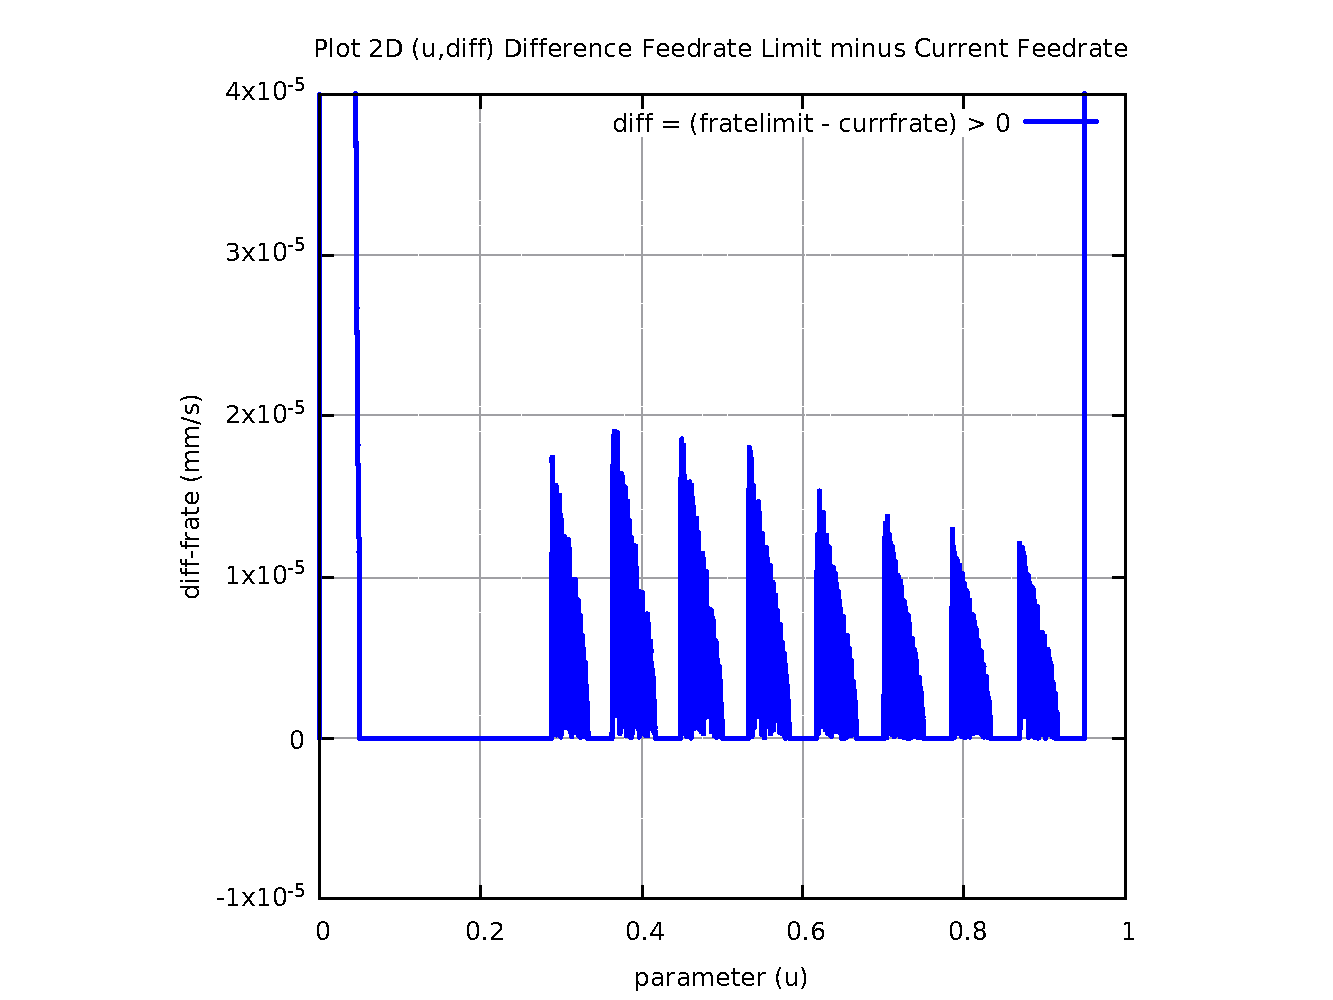
\includegraphics[width=1.00\textwidth]{Chap4/appendix/app-Snailshell/plots/12-img-Snailshell-FeedRateLimit-minus-CurrFeedRate.pdf}
\end{figure}

%% ==================================================
\clearpage
\pagebreak

\begin{figure}
	\caption     {Snailshell FC20-Nominal X and Y Feedrate Profiles}
	\label{13-img-Snailshell-FC20-Nominal-X-and-Y-Feedrate-Profiles.pdf}
	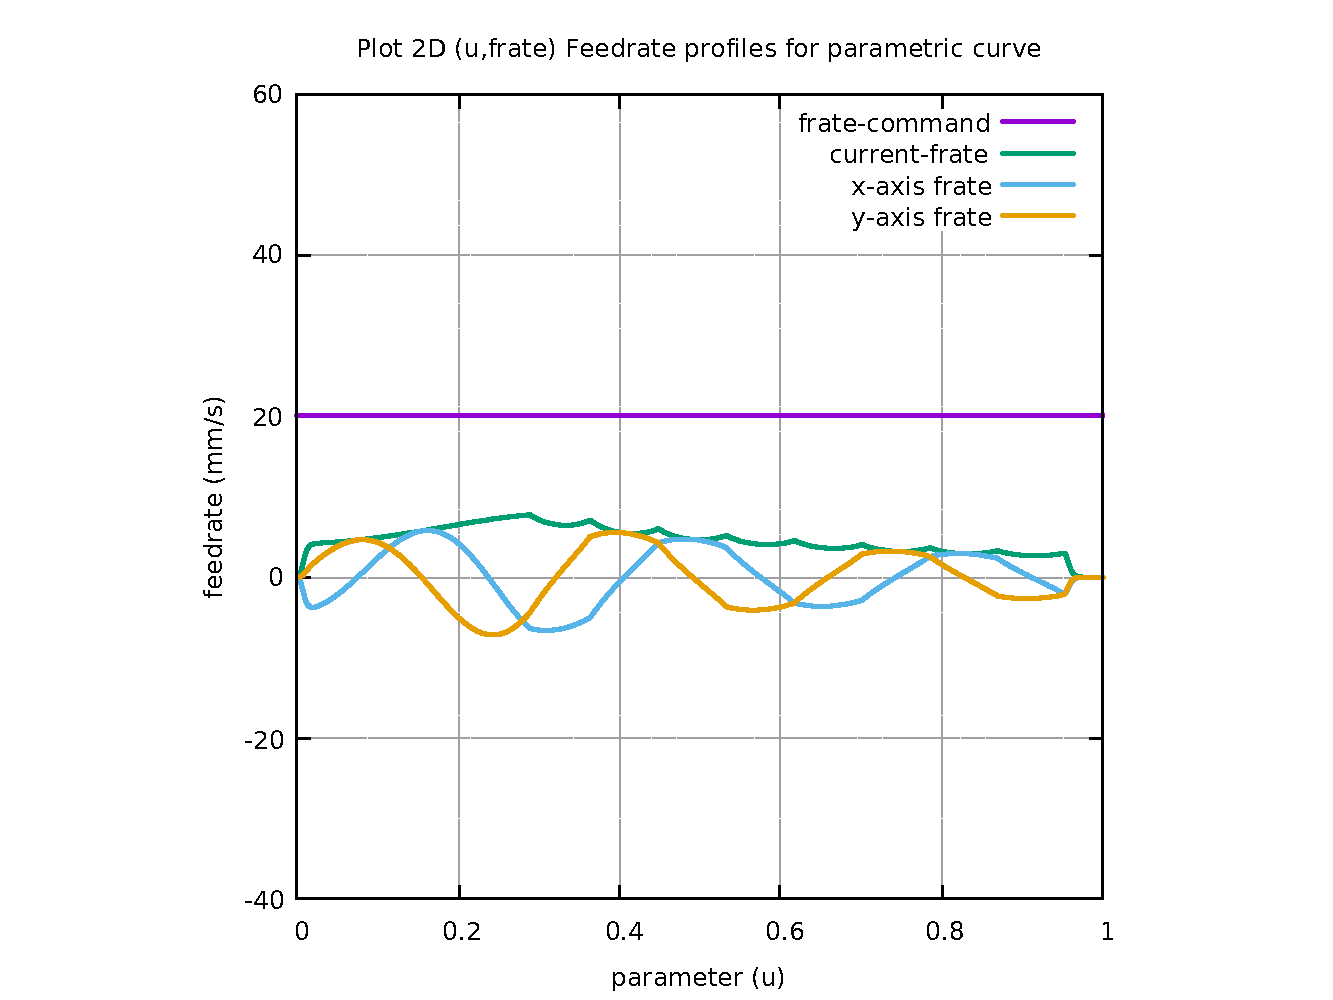
\includegraphics[width=1.00\textwidth]{Chap4/appendix/app-Snailshell/plots/13-img-Snailshell-FC20-Nominal-X-and-Y-Feedrate-Profiles.pdf}
\end{figure}


\begin{figure}
	\caption     {Snailshell FC20 Nominal Tangential Acceleration}
	\label{14-img-Snailshell-FC20-Nominal-Tangential-Acceleration.pdf}
	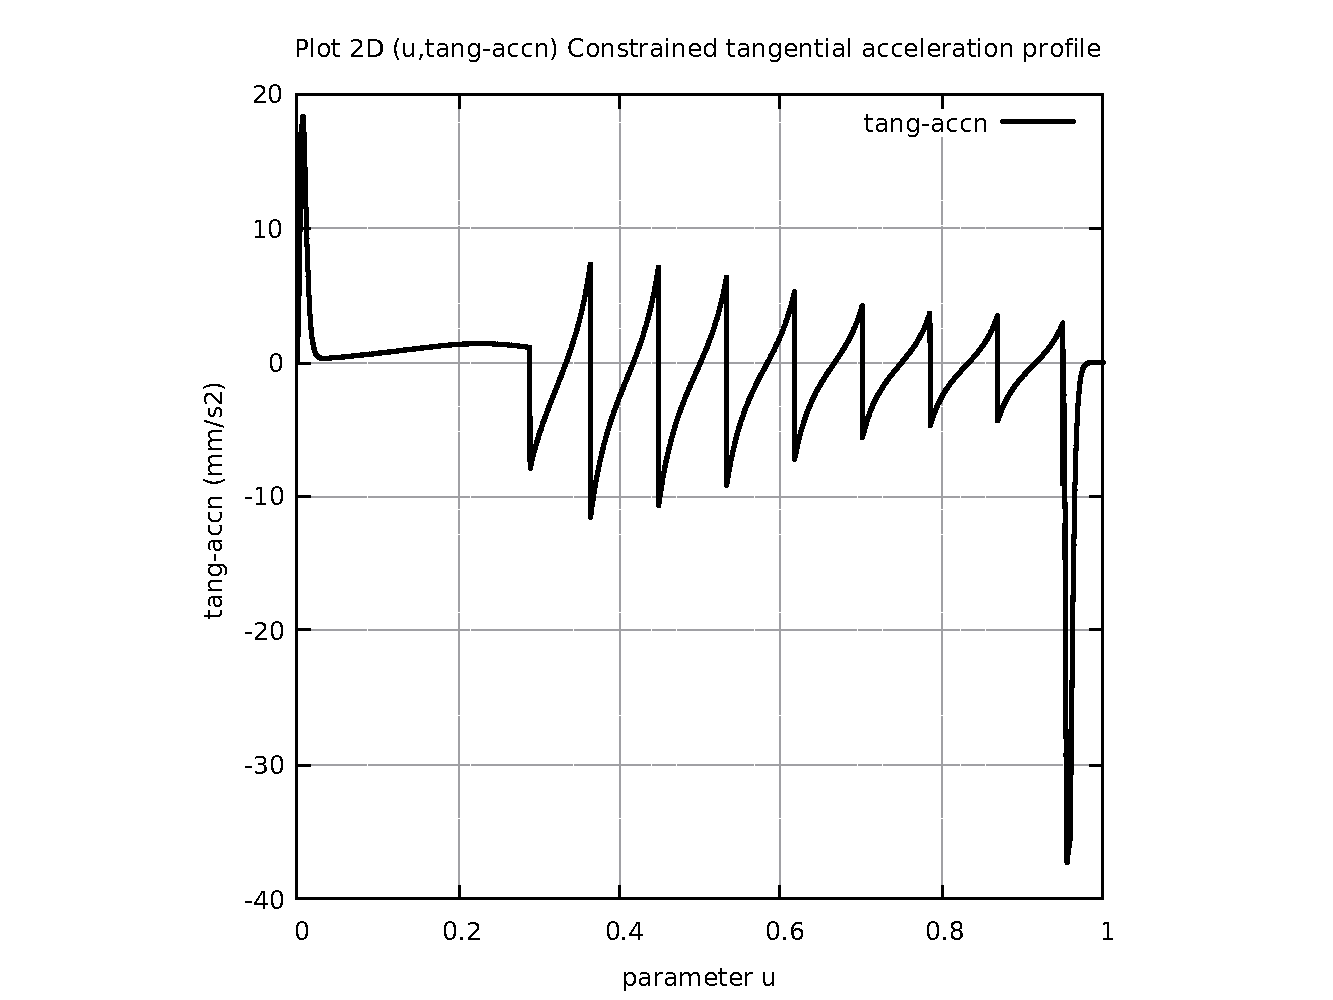
\includegraphics[width=1.00\textwidth]{Chap4/appendix/app-Snailshell/plots/14-img-Snailshell-FC20-Nominal-Tangential-Acceleration.pdf}
\end{figure}

%% ==================================================
\clearpage
\pagebreak

\begin{figure}
	\caption     {Snailshell FC20 Nominal Rising S-Curve Profile}
	\label{15-img-Snailshell-FC20-Nominal-Rising-S-Curve-Profile.pdf}
	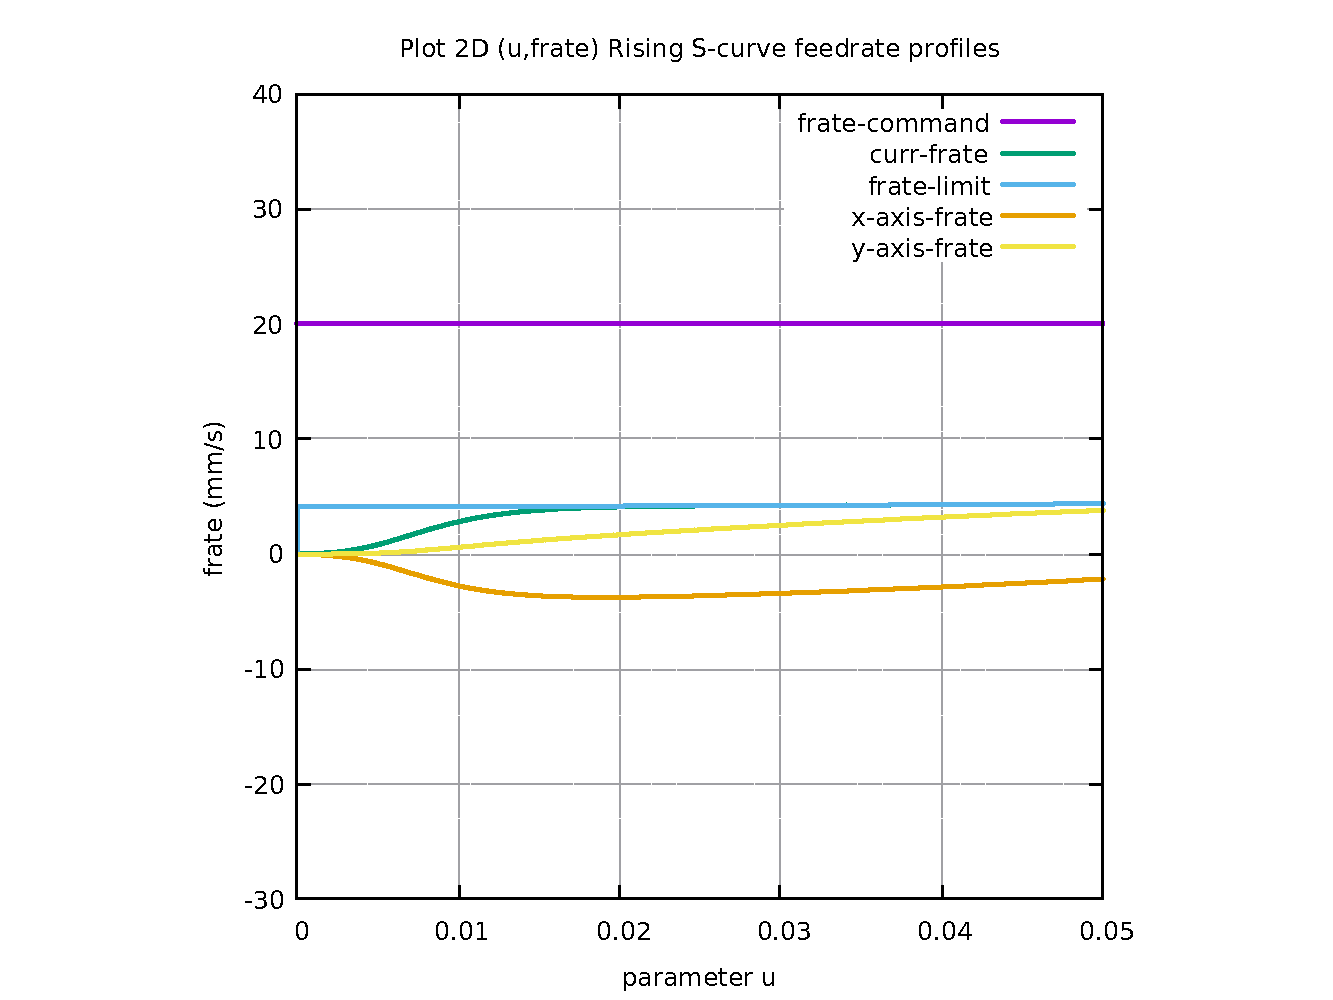
\includegraphics[width=1.00\textwidth]{Chap4/appendix/app-Snailshell/plots/15-img-Snailshell-FC20-Nominal-Rising-S-Curve-Profile.pdf}
\end{figure}


\begin{figure}
	\caption     {Snailshell FC20 Nominal Falling S-Curve Profile}
	\label{16-img-Snailshell-FC20-Nominal-Falling-S-Curve-Profile.pdf}
	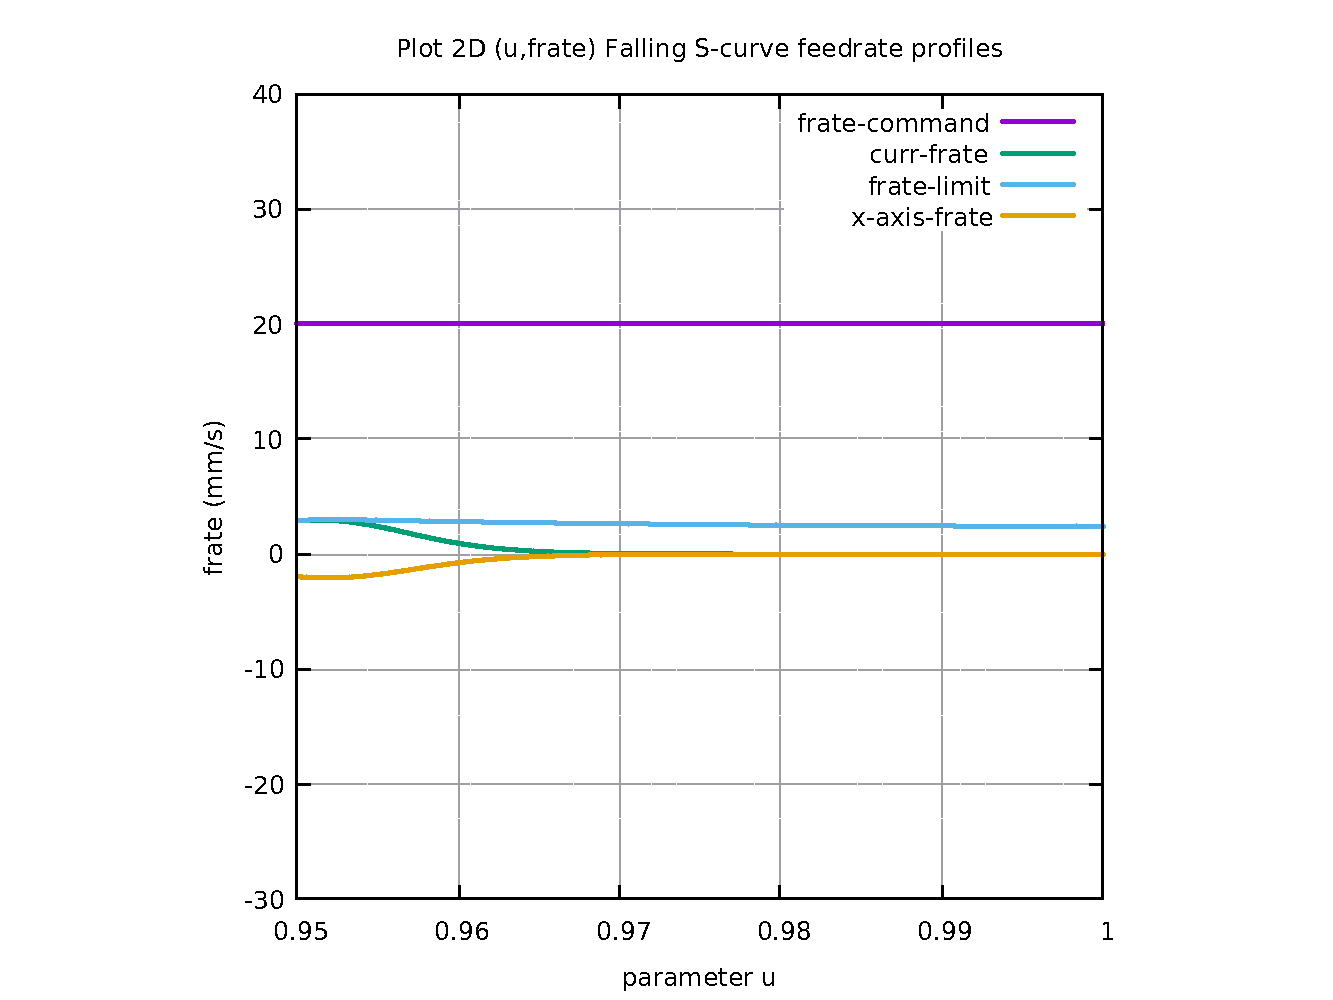
\includegraphics[width=1.00\textwidth]{Chap4/appendix/app-Snailshell/plots/16-img-Snailshell-FC20-Nominal-Falling-S-Curve-Profile.pdf}
\end{figure}

%% ==================================================
\clearpage
\pagebreak

\begin{figure}
	\caption     {Snailshell FC10 Colored Feedrate Profile data ngcode}
	\label{17-img-Snailshell-FC10-Colored-Feedrate-Profile-data_ngcode.png}
	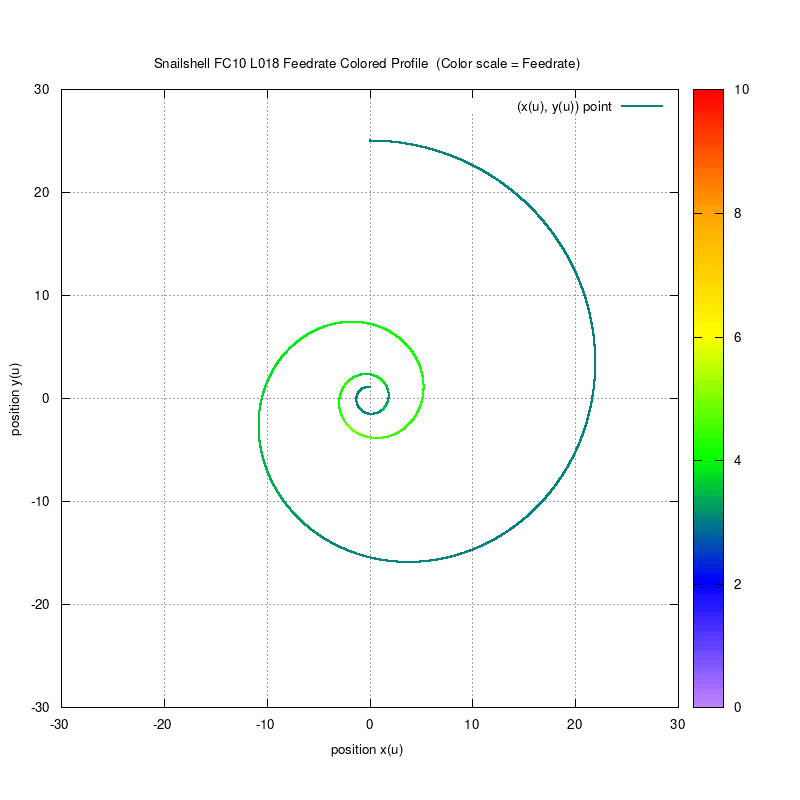
\includegraphics[width=0.75\textwidth]{Chap4/appendix/app-Snailshell/plots/17-img-Snailshell-FC10-Colored-Feedrate-Profile-data_ngcode.png}
\end{figure}


\begin{figure}
	\caption     {Snailshell FC20 Colored Feedrate Profile data ngcode}
	\label{18-img-Snailshell-FC20-Colored-Feedrate-Profile-data_ngcode.png}
	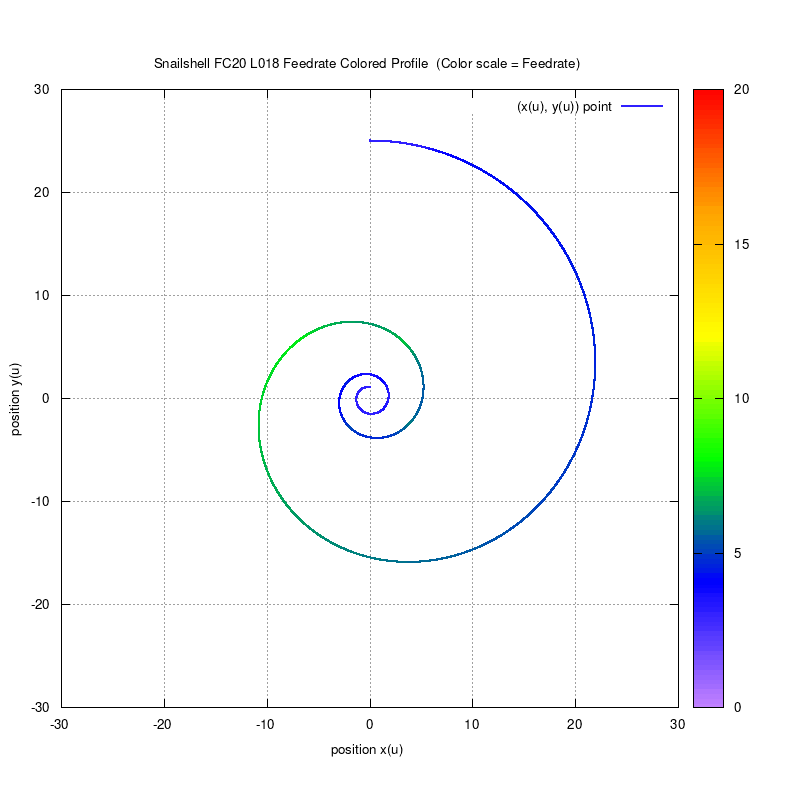
\includegraphics[width=0.75\textwidth]{Chap4/appendix/app-Snailshell/plots/18-img-Snailshell-FC20-Colored-Feedrate-Profile-data_ngcode.png}
\end{figure}

%% ==================================================
\clearpage
\pagebreak

\begin{figure}
	\caption     {Snailshell FC30 Colored Feedrate Profile data ngcode}
	\label{19-img-Snailshell-FC30-Colored-Feedrate-Profile-data_ngcode.png}
	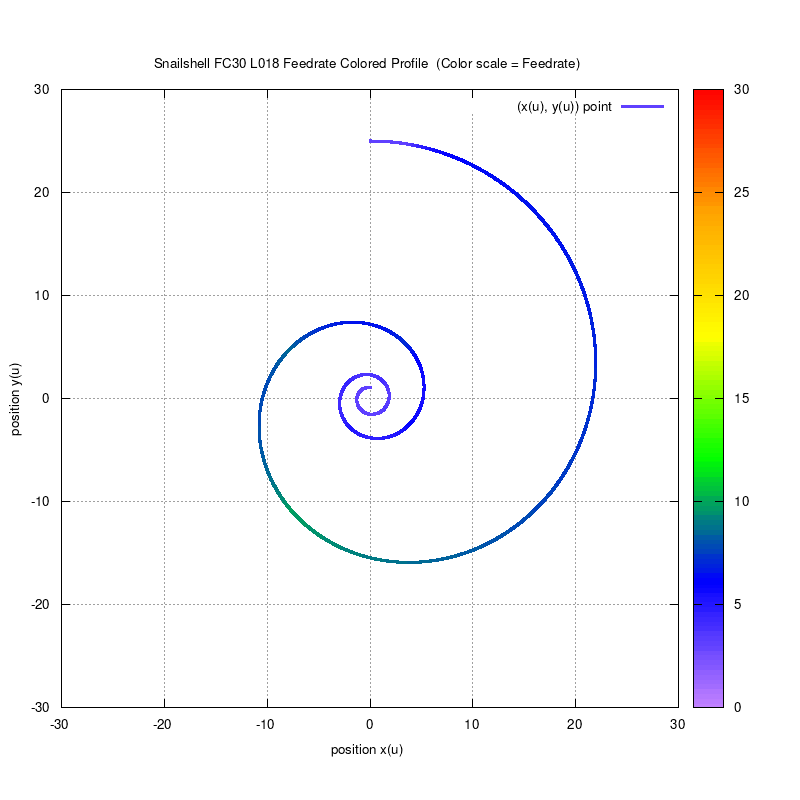
\includegraphics[width=0.75\textwidth]{Chap4/appendix/app-Snailshell/plots/19-img-Snailshell-FC30-Colored-Feedrate-Profile-data_ngcode.png}
\end{figure}


\begin{figure}
	\caption     {Snailshell FC40 Colored Feedrate Profile data ngcode}
	\label{20-img-Snailshell-FC40-Colored-Feedrate-Profile-data_ngcode.png}
	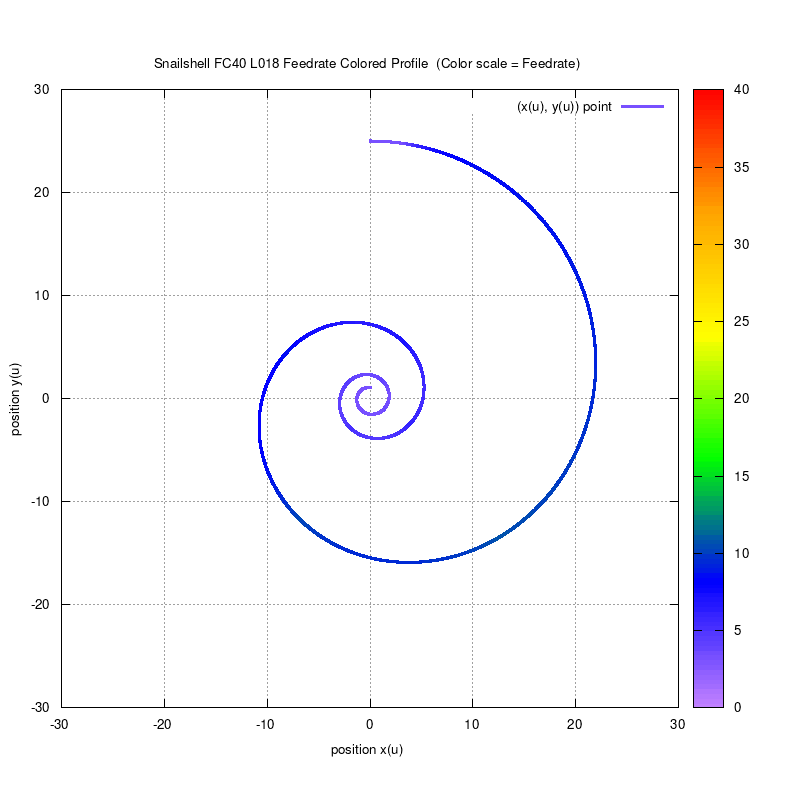
\includegraphics[width=0.75\textwidth]{Chap4/appendix/app-Snailshell/plots/20-img-Snailshell-FC40-Colored-Feedrate-Profile-data_ngcode.png}
\end{figure}

%% ==================================================
\clearpage
\pagebreak

\begin{figure}
	\caption     {Snailshell FC10 Tangential Acceleration}
	\label{21-img-Snailshell-FC10-Tangential-Acceleration.pdf}
	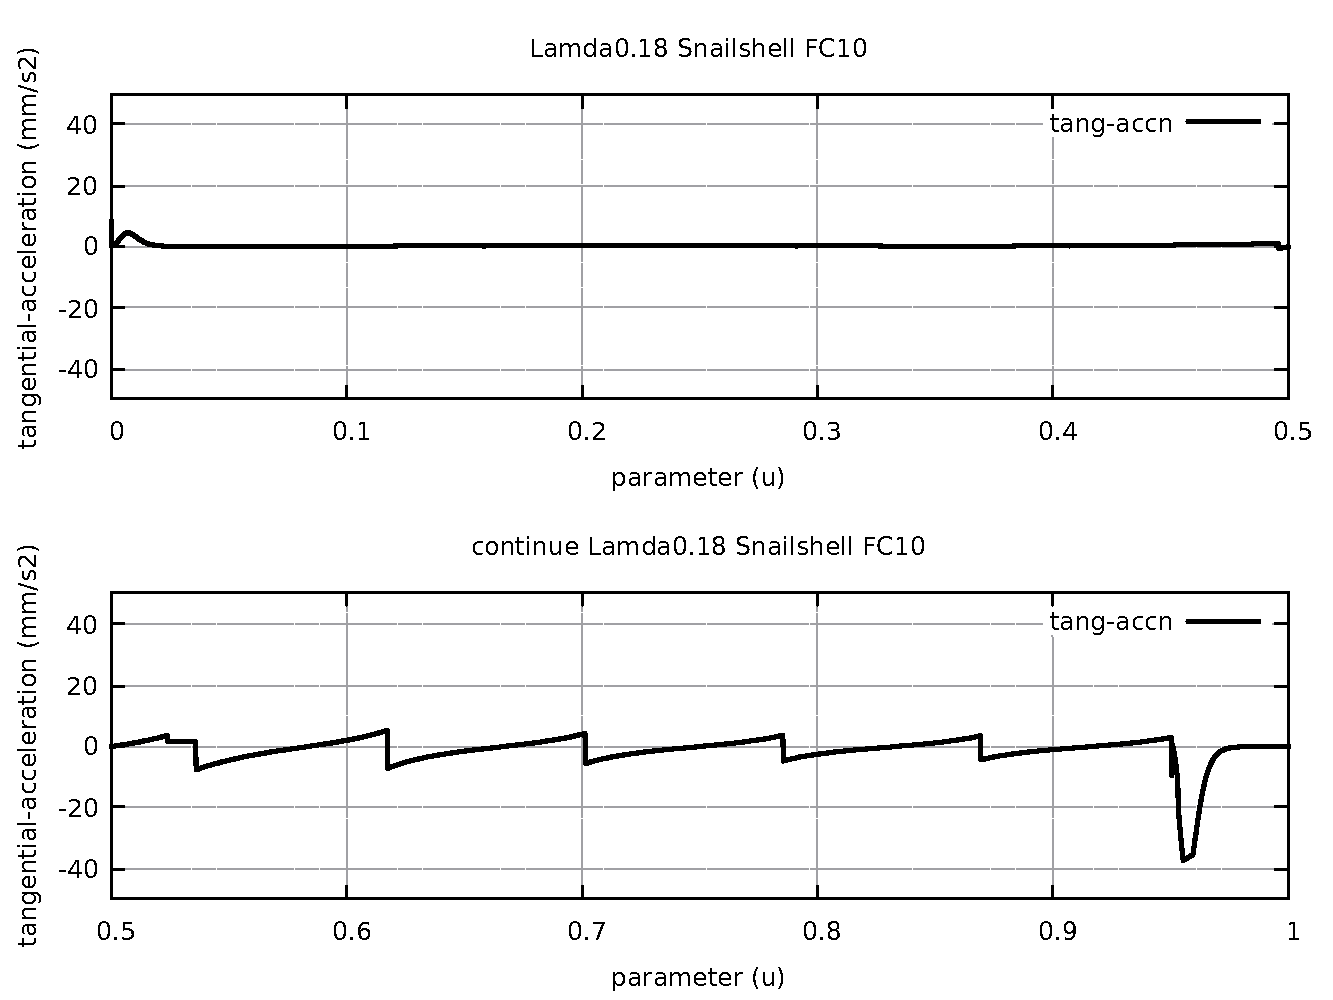
\includegraphics[width=1.00\textwidth]{Chap4/appendix/app-Snailshell/plots/21-img-Snailshell-FC10-Tangential-Acceleration.pdf}
\end{figure}


\begin{figure}
	\caption     {Snailshell FC20 Tangential Acceleration}
	\label{22-img-Snailshell-FC20-Tangential-Acceleration.pdf}
	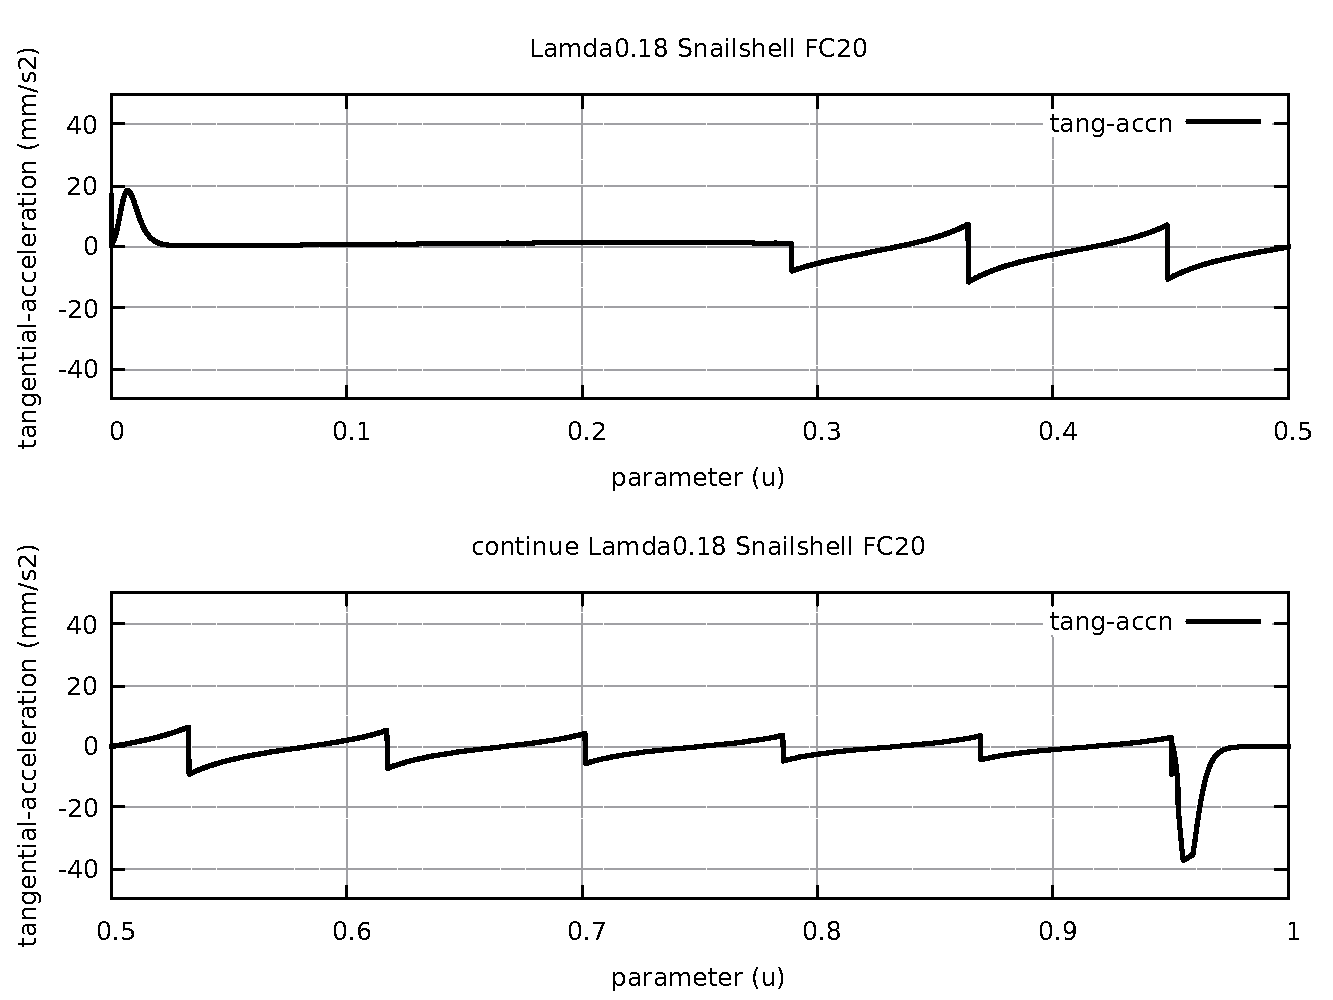
\includegraphics[width=1.00\textwidth]{Chap4/appendix/app-Snailshell/plots/22-img-Snailshell-FC20-Tangential-Acceleration.pdf}
\end{figure}

%% ==================================================
\clearpage
\pagebreak

\begin{figure}
	\caption     {Snailshell FC30 Tangential Acceleration}
	\label{23-img-Snailshell-FC30-Tangential-Acceleration.pdf}
	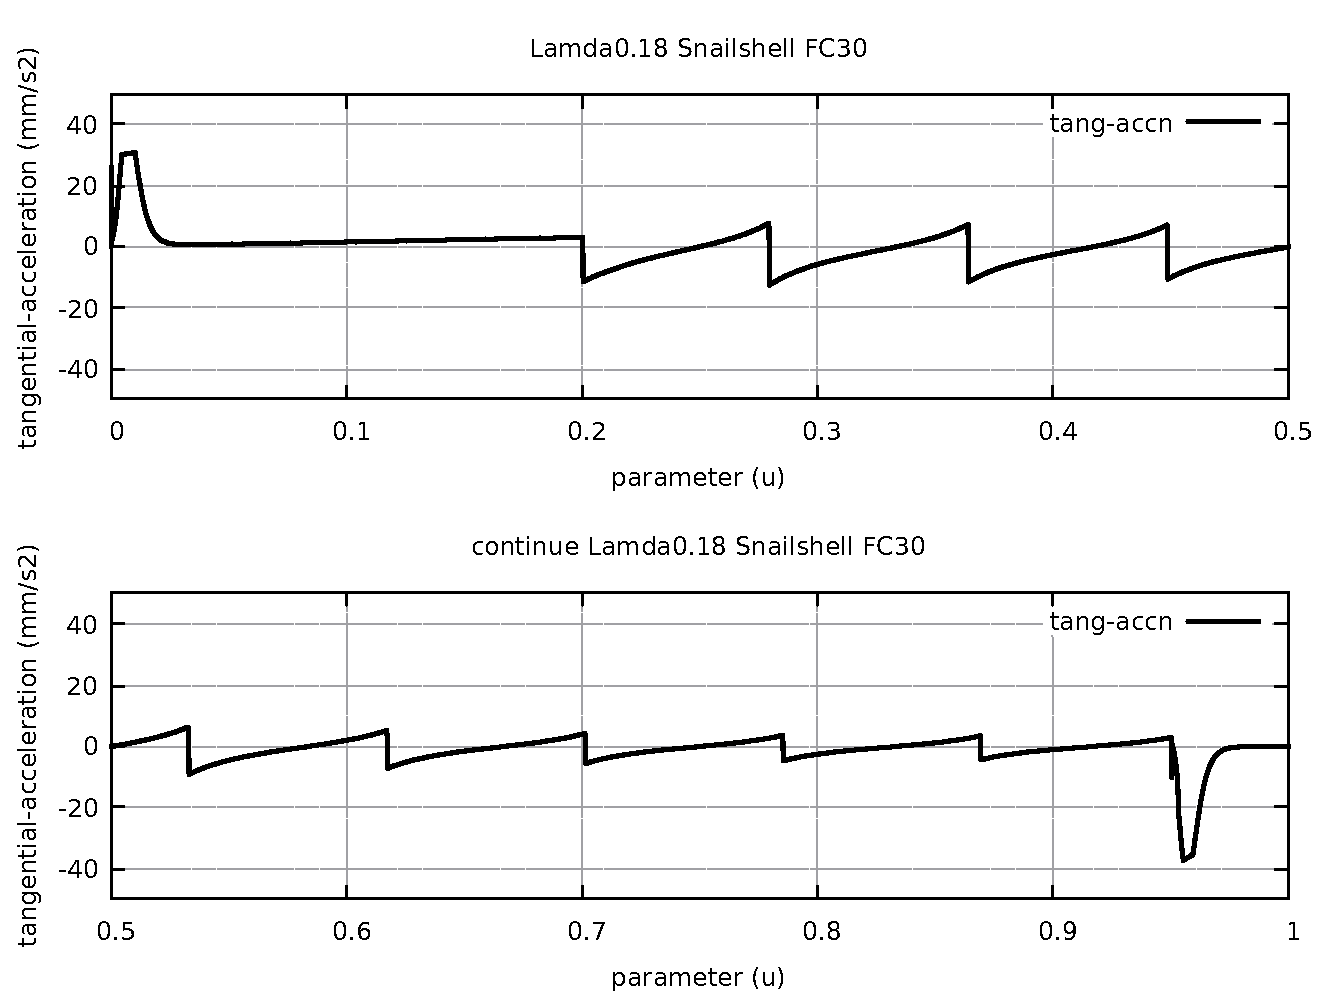
\includegraphics[width=1.00\textwidth]{Chap4/appendix/app-Snailshell/plots/23-img-Snailshell-FC30-Tangential-Acceleration.pdf}
\end{figure}


\begin{figure}
	\caption     {Snailshell FC40 Tangential Acceleration}
	\label{24-img-Snailshell-FC40-Tangential-Acceleration.pdf}
	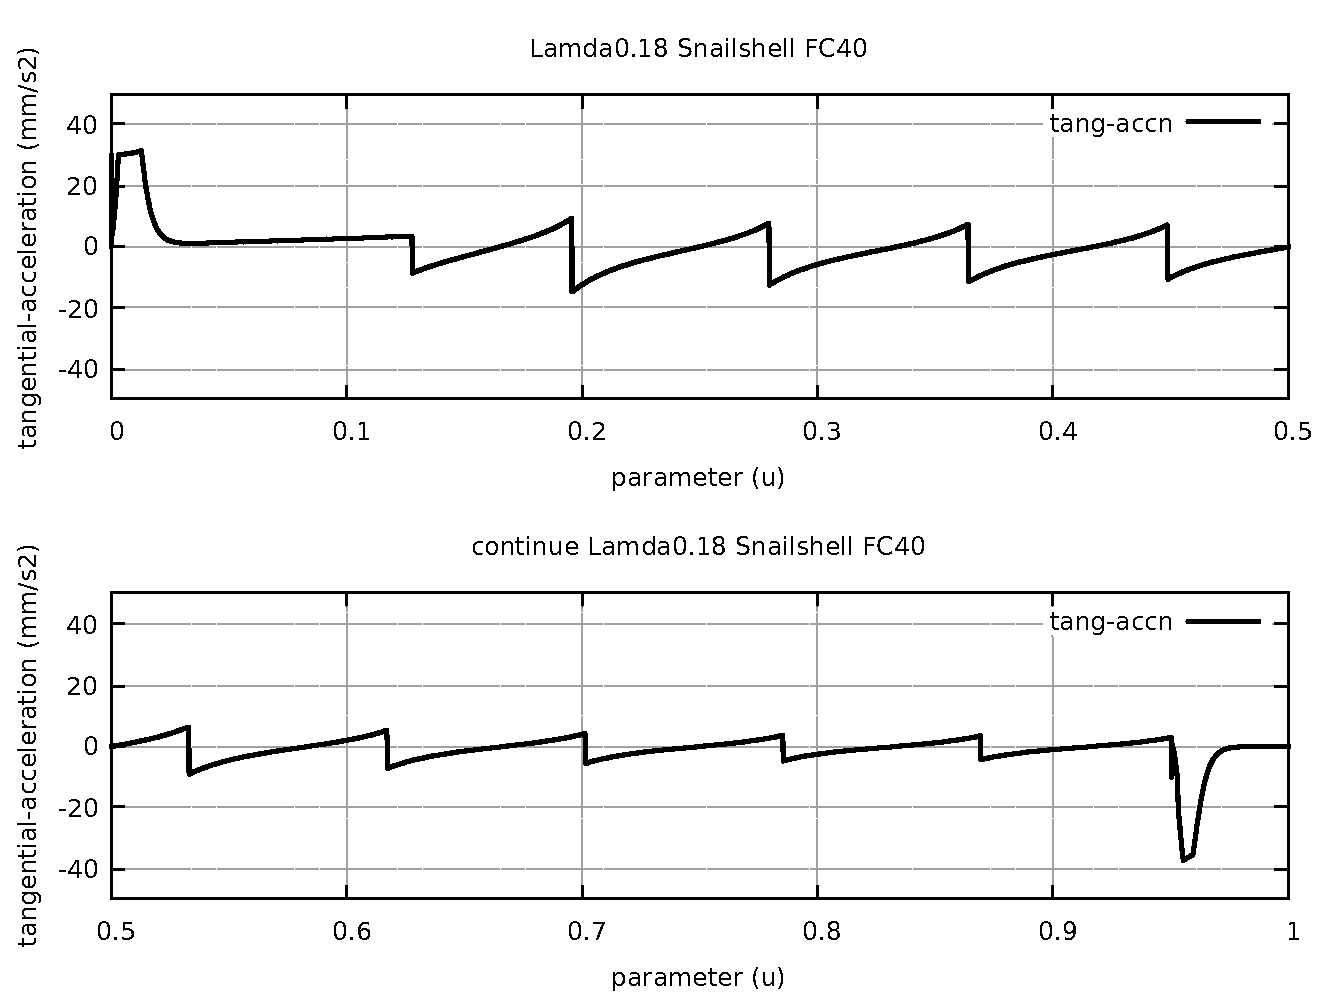
\includegraphics[width=1.00\textwidth]{Chap4/appendix/app-Snailshell/plots/24-img-Snailshell-FC40-Tangential-Acceleration.pdf}
\end{figure}

%% ==================================================
\clearpage
\pagebreak

\begin{figure}
	\caption     {Snailshell FC20 Nominal Separation NAL and NCL}
	\label{25-img-Snailshell-FC20-Nominal-Separation-NAL-and-NCL.pdf}
	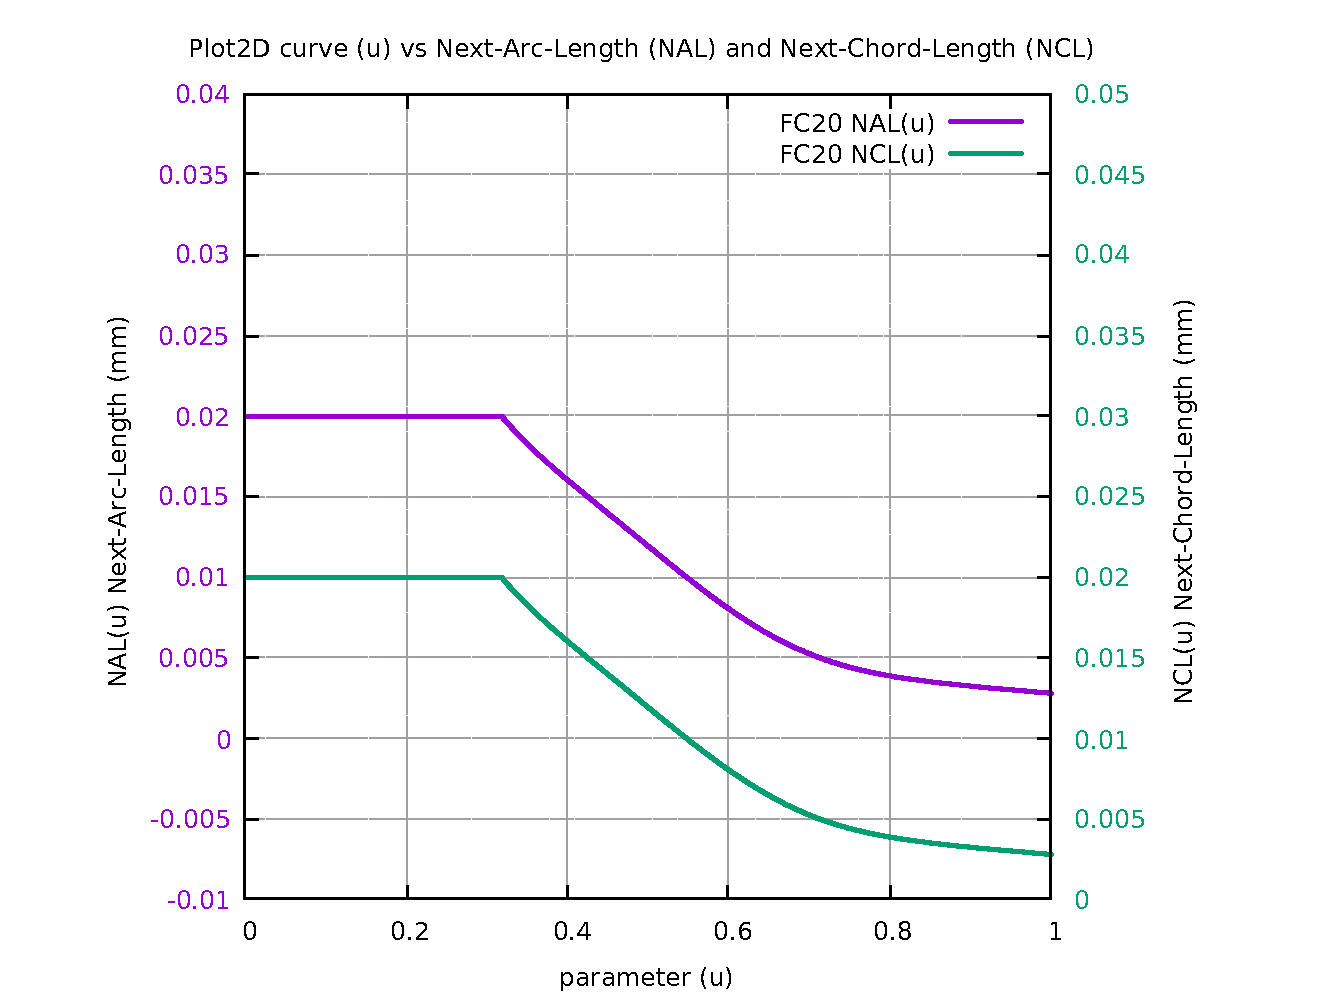
\includegraphics[width=1.00\textwidth]{Chap4/appendix/app-Snailshell/plots/25-img-Snailshell-FC20-Nominal-Separation-NAL-and-NCL.pdf}
\end{figure}


\begin{figure}
	\caption     {Snailshell Difference SAL minus SCL for FC10 FC20 FC30 FC40}
	\label{26-img-Snailshell-Difference-SAL-minus-SCL-for-FC10-FC20-FC30-FC40.pdf}
	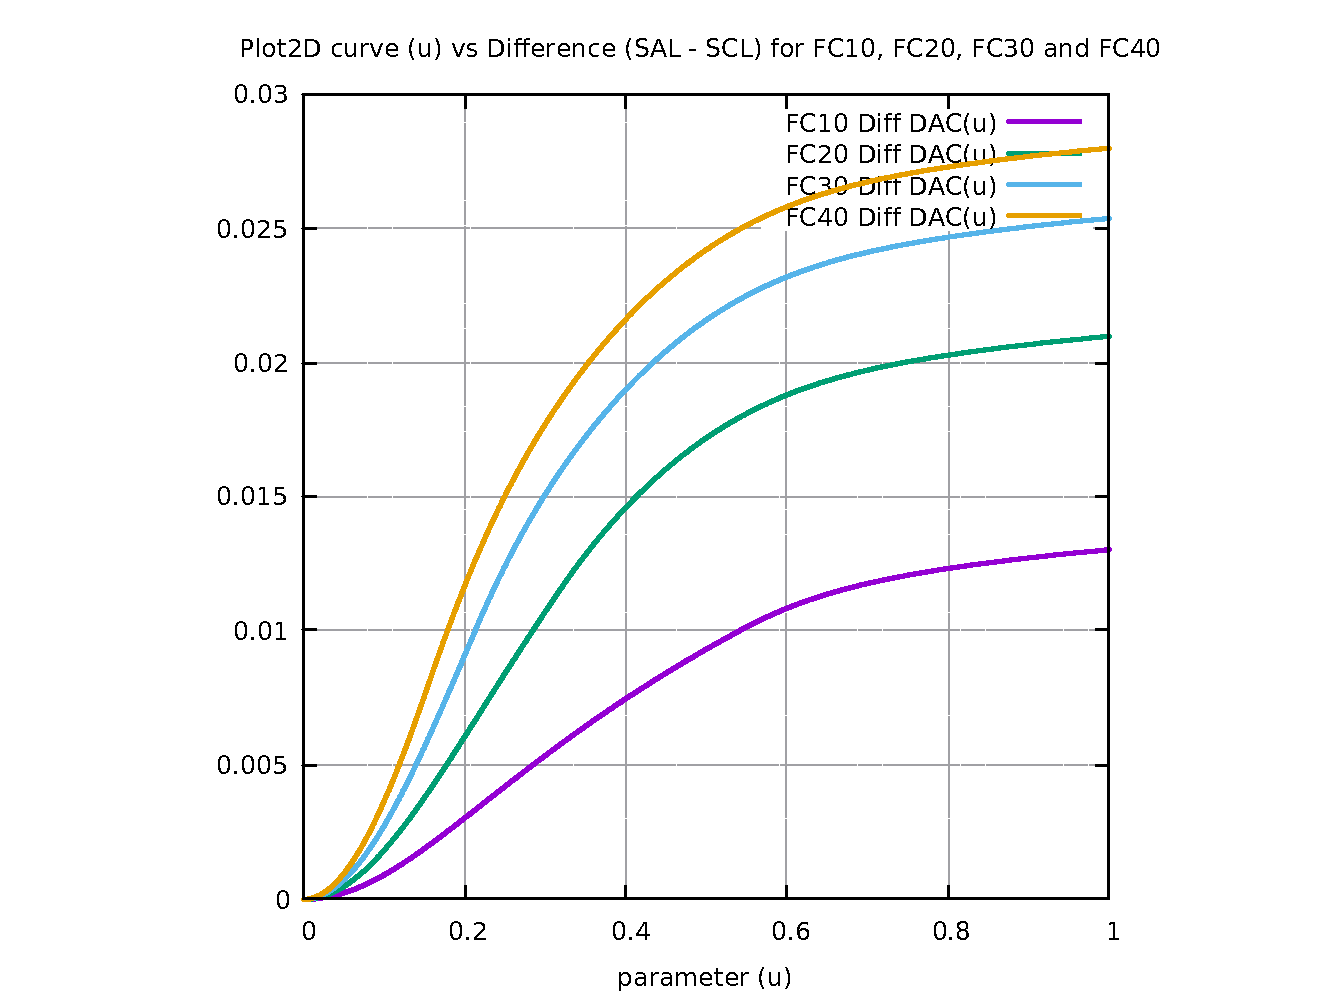
\includegraphics[width=1.00\textwidth]{Chap4/appendix/app-Snailshell/plots/26-img-Snailshell-Difference-SAL-minus-SCL-for-FC10-FC20-FC30-FC40.pdf}
\end{figure}


%% ==================================================
\clearpage
\pagebreak

\begin{figure}
	\caption     {Snailshell FC10 FrateCmd CurrFrate X-Frate Y-Frate}
	\label{27-img-Snailshell-FC10-FrateCmd-CurrFrate-X-Frate-Y-Frate.pdf}
	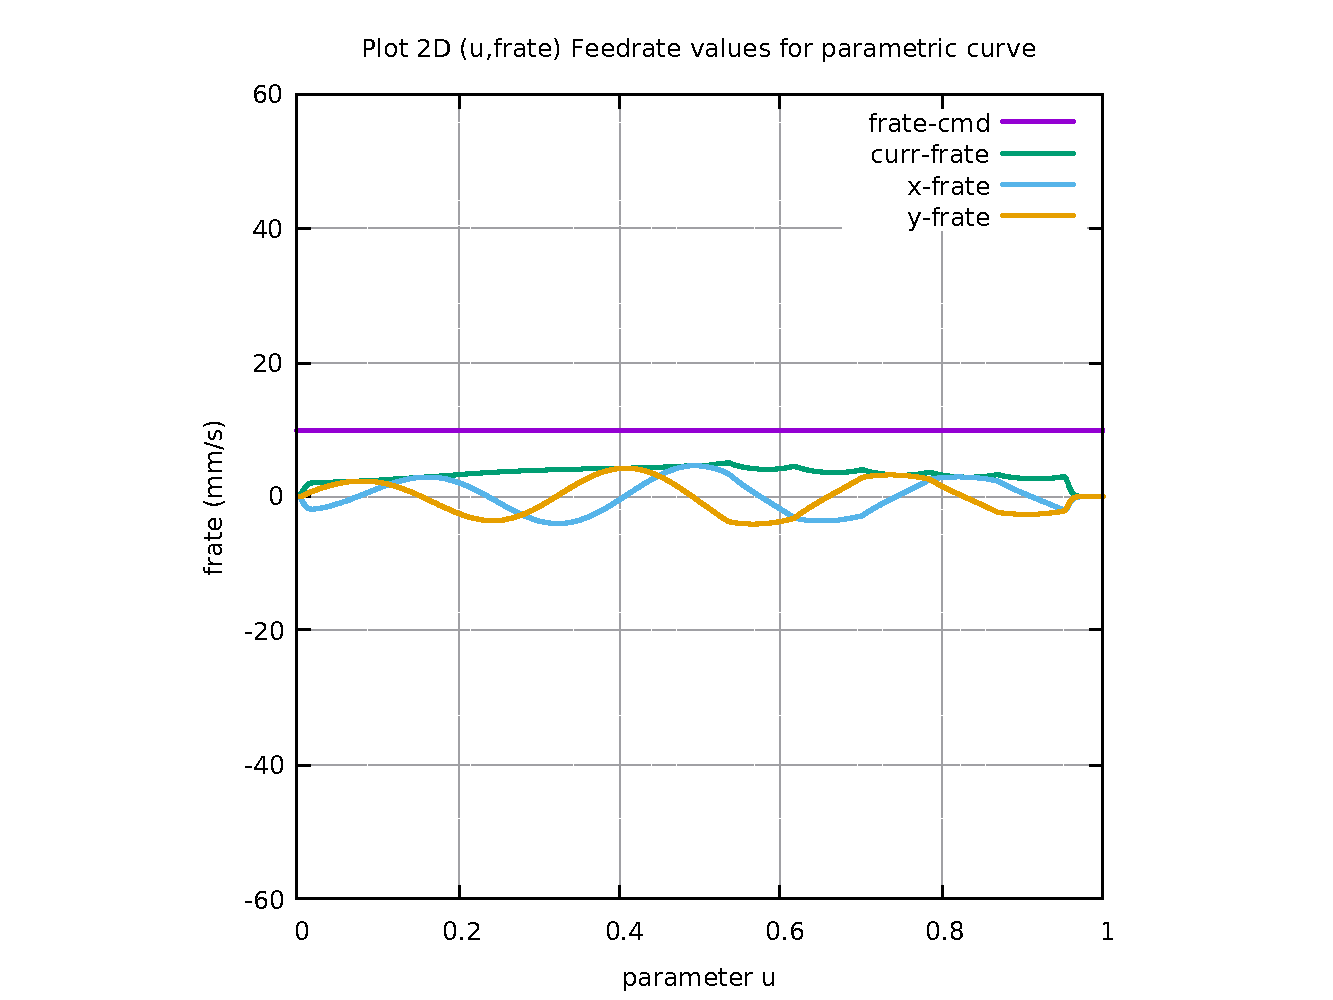
\includegraphics[width=1.00\textwidth]{Chap4/appendix/app-Snailshell/plots/27-img-Snailshell-FC10-FrateCmd-CurrFrate-X-Frate-Y-Frate.pdf}
\end{figure}


\begin{figure}
	\caption     {Snailshell FC20 FrateCmd CurrFrate X-Frate Y-Frate}
	\label{28-img-Snailshell-FC20-FrateCmd-CurrFrate-X-Frate-Y-Frate.pdf}
	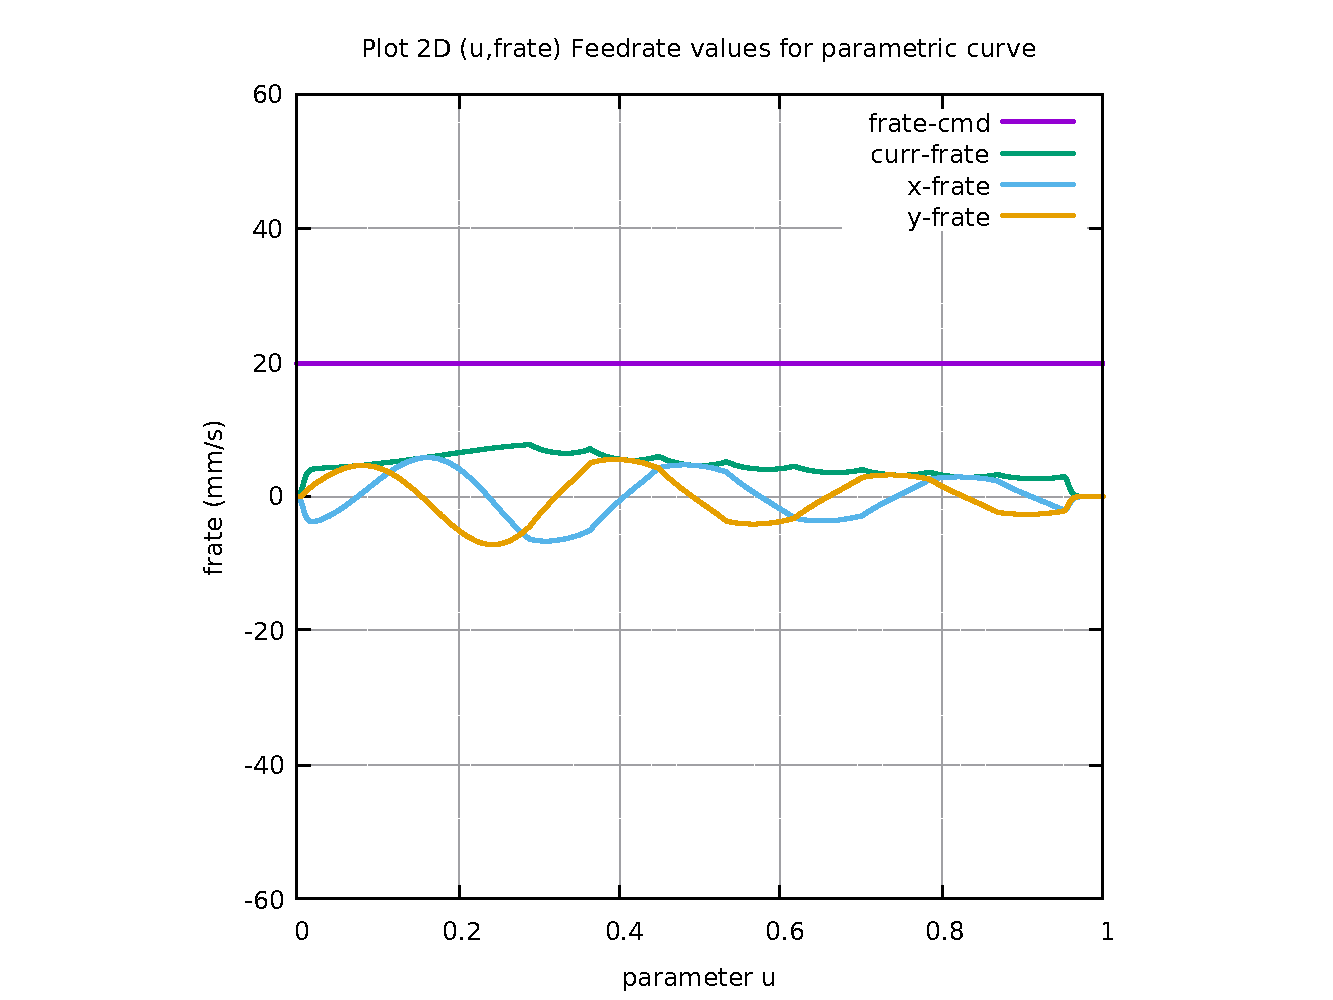
\includegraphics[width=1.00\textwidth]{Chap4/appendix/app-Snailshell/plots/28-img-Snailshell-FC20-FrateCmd-CurrFrate-X-Frate-Y-Frate.pdf}
\end{figure}


%% ==================================================
\clearpage
\pagebreak

\begin{figure}
	\caption     {Snailshell FC30 FrateCmd CurrFrate X-Frate Y-Frate}
	\label{29-img-Snailshell-FC30-FrateCmd-CurrFrate-X-Frate-Y-Frate.pdf}
	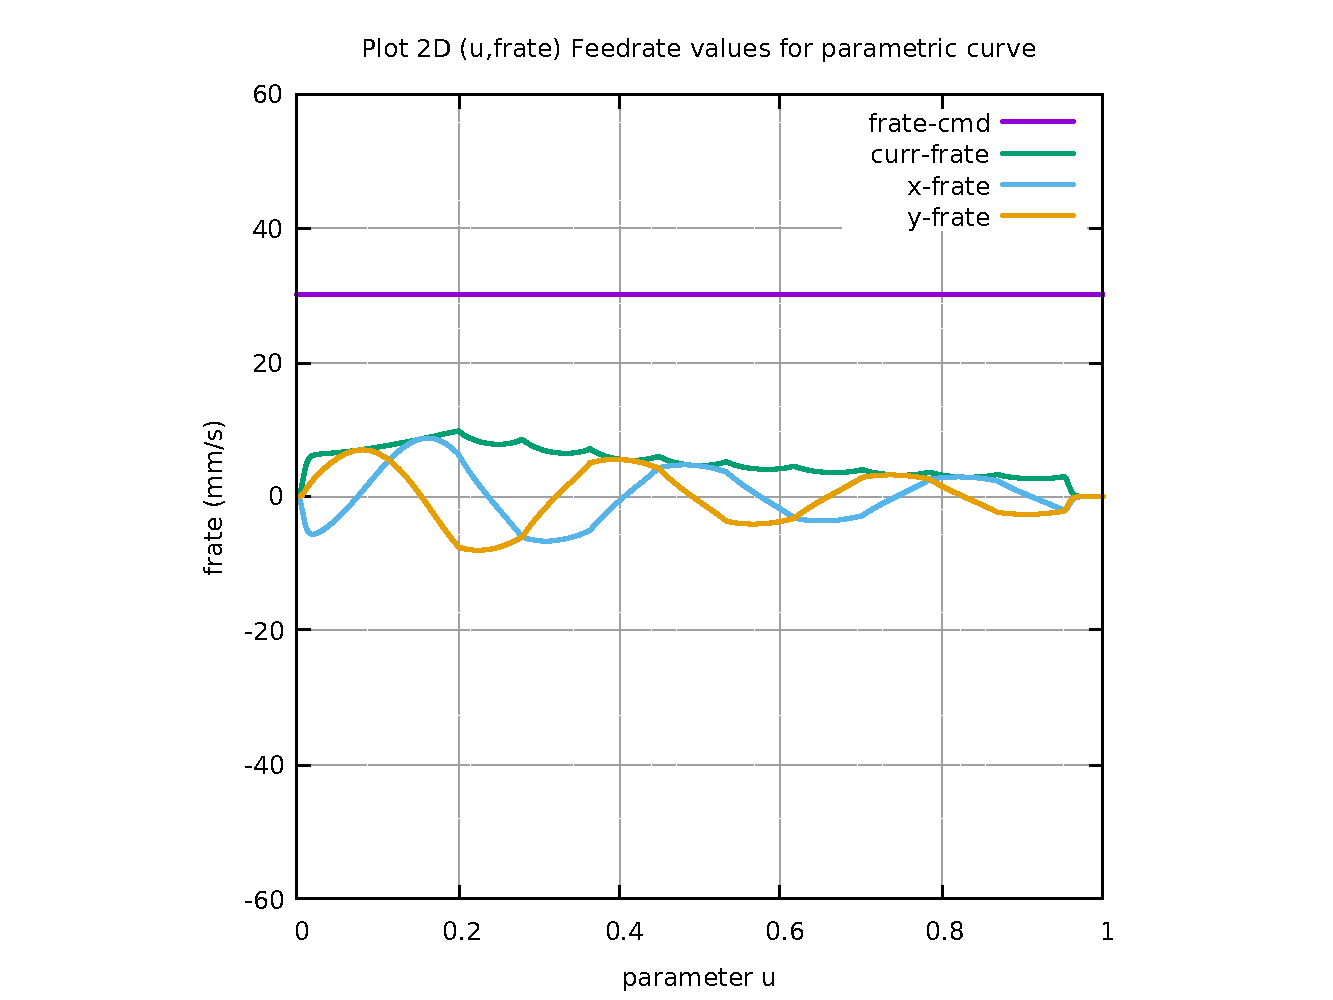
\includegraphics[width=1.00\textwidth]{Chap4/appendix/app-Snailshell/plots/29-img-Snailshell-FC30-FrateCmd-CurrFrate-X-Frate-Y-Frate.pdf}
\end{figure}


\begin{figure}
	\caption     {Snailshell FC40 FrateCmd CurrFrate X-Frate Y-Frate}
	\label{30-img-Snailshell-FC40-FrateCmd-CurrFrate-X-Frate-Y-Frate.pdf}
	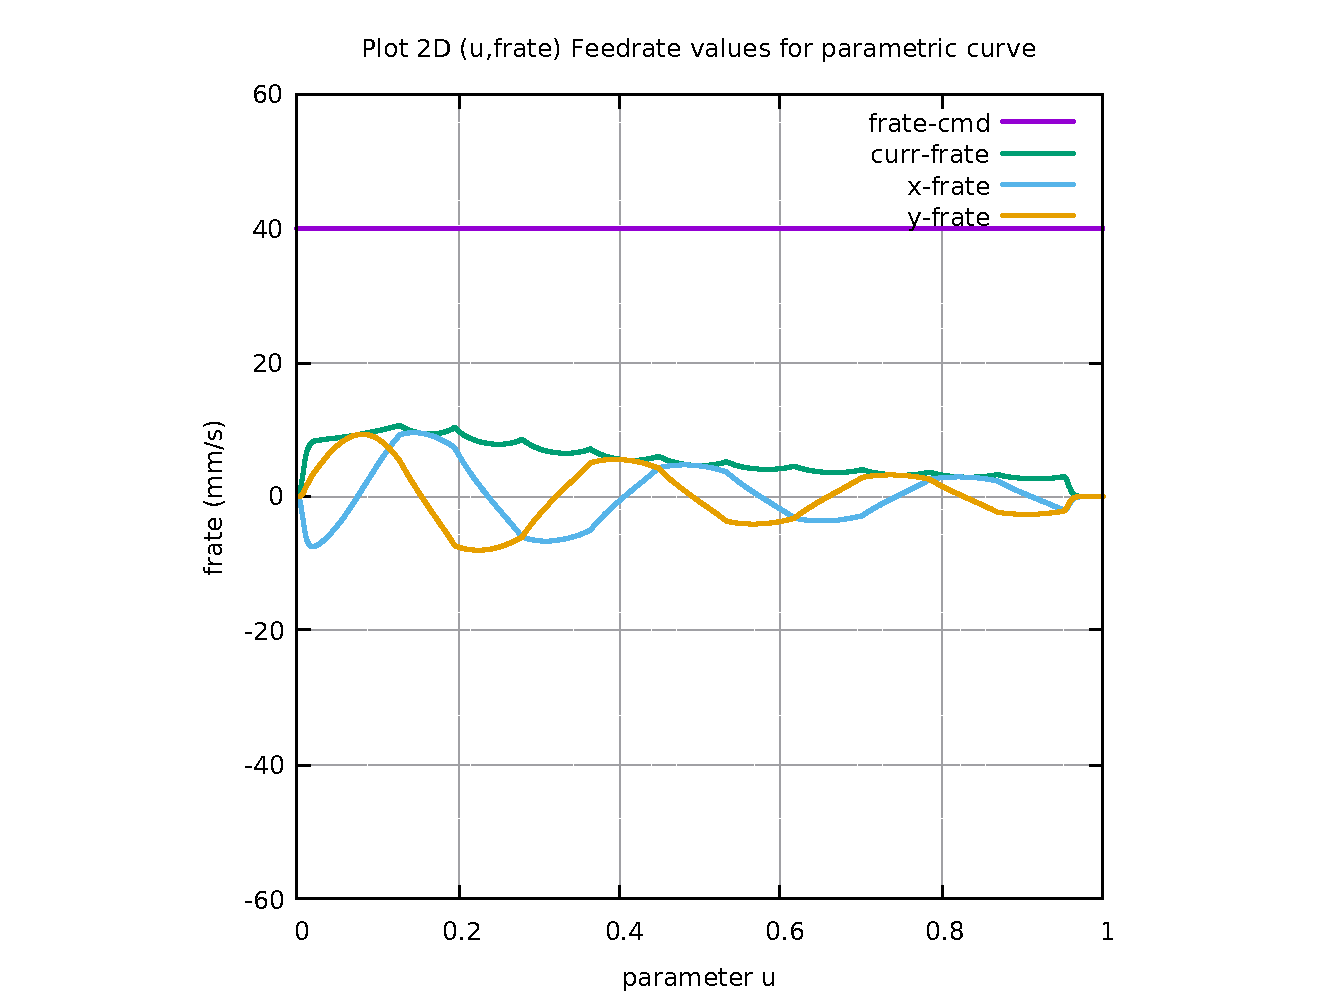
\includegraphics[width=1.00\textwidth]{Chap4/appendix/app-Snailshell/plots/30-img-Snailshell-FC40-FrateCmd-CurrFrate-X-Frate-Y-Frate.pdf}
\end{figure}


%% ==================================================
\clearpage
\pagebreak

\begin{figure}
	\caption     {Snailshell FC10 Four Components FeedrateLimit}
	\label{31-img-Snailshell-FC10-Four-Components-FeedrateLimit.pdf}
	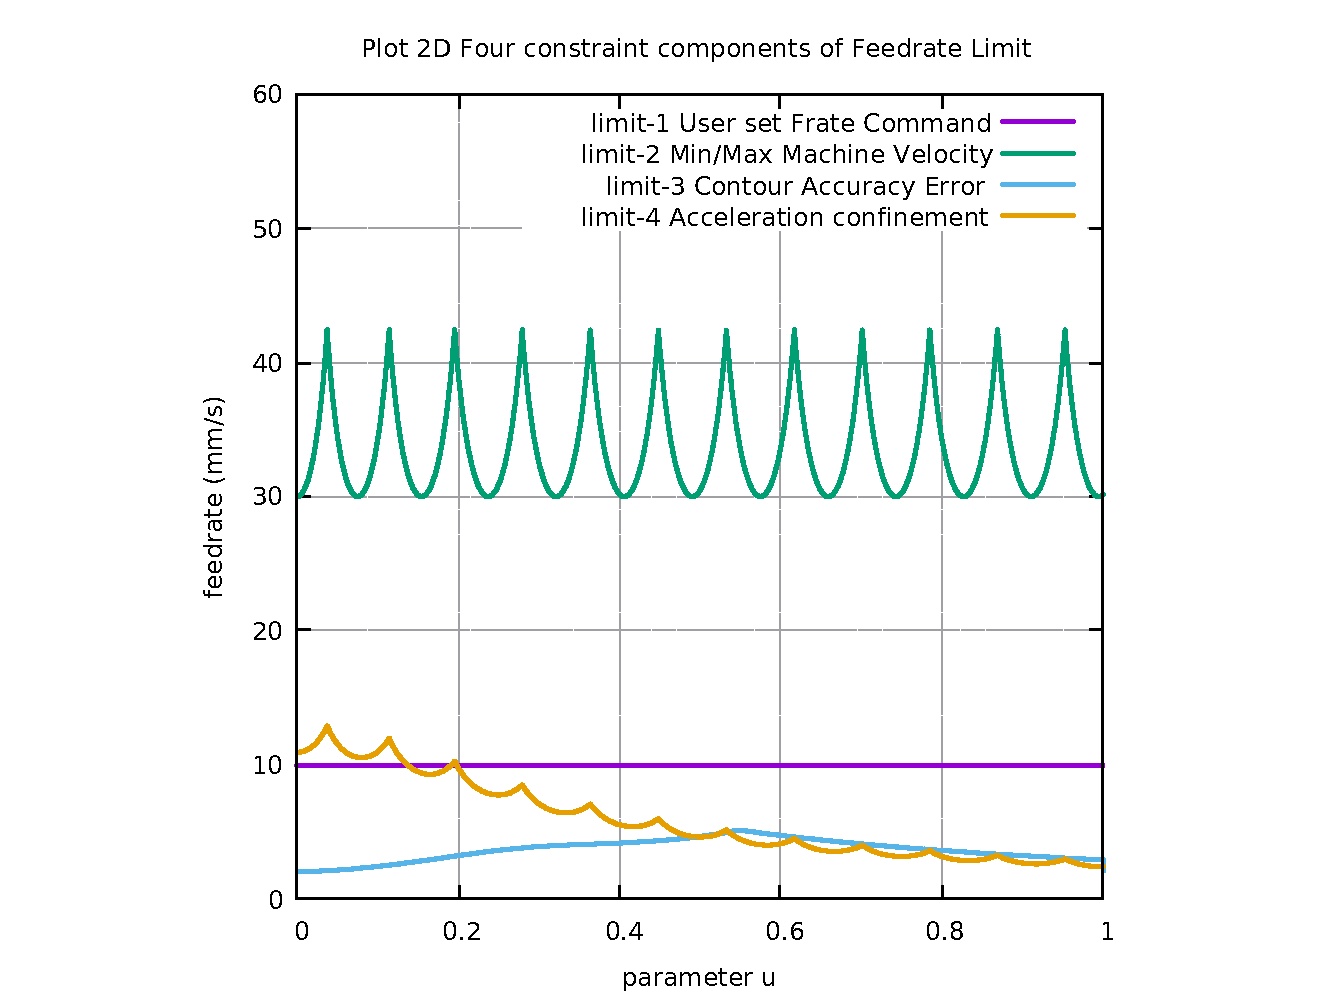
\includegraphics[width=1.00\textwidth]{Chap4/appendix/app-Snailshell/plots/31-img-Snailshell-FC10-Four-Components-FeedrateLimit.pdf}
\end{figure}


\begin{figure}
	\caption     {Snailshell FC20 Four Components FeedrateLimit}
	\label{32-img-Snailshell-FC20-Four-Components-FeedrateLimit.pdf}
	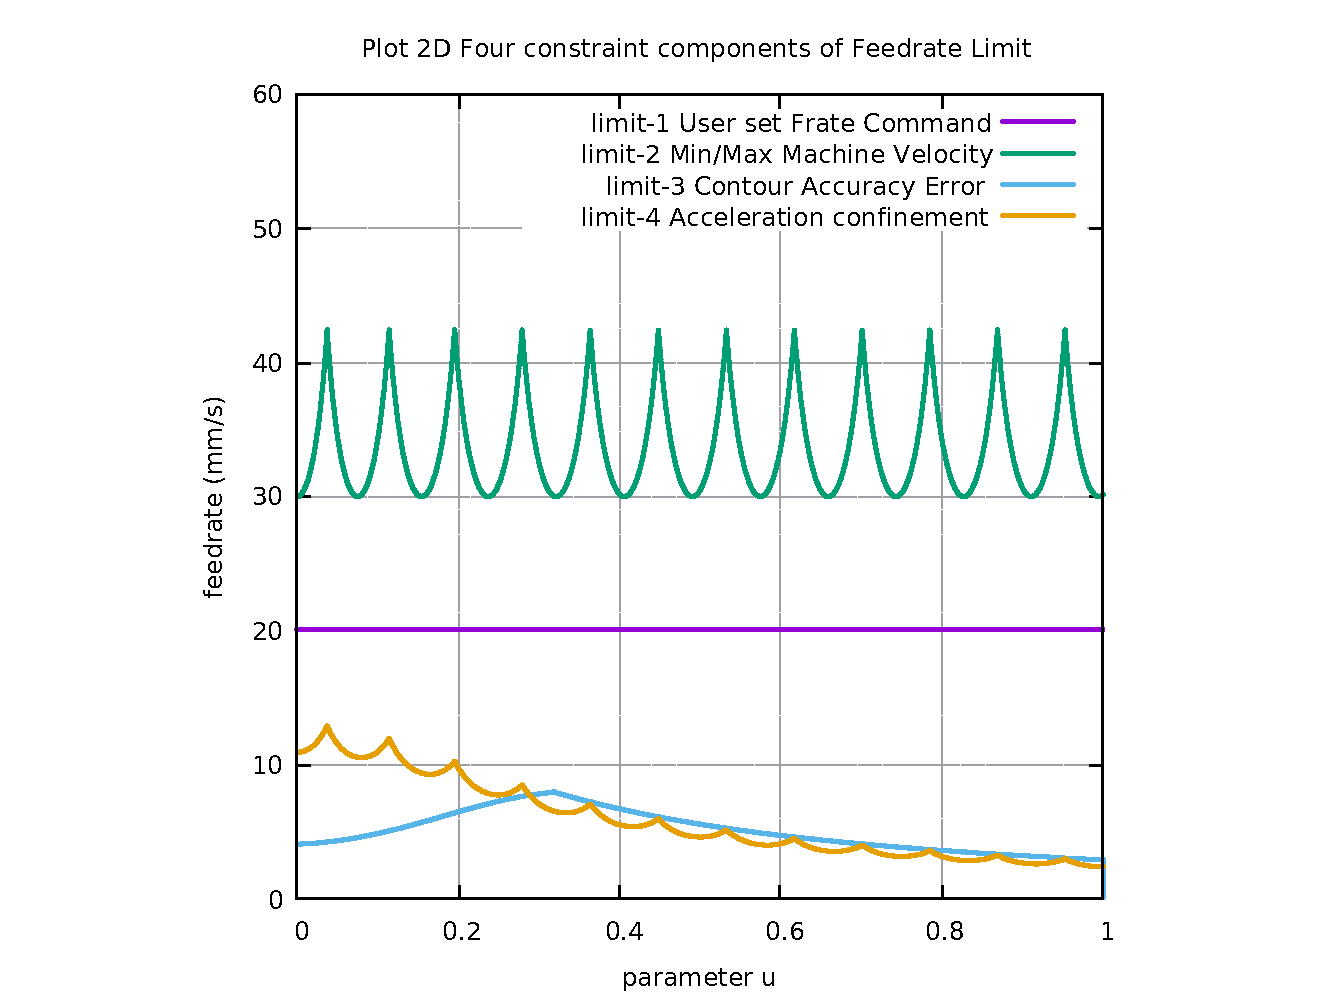
\includegraphics[width=1.00\textwidth]{Chap4/appendix/app-Snailshell/plots/32-img-Snailshell-FC20-Four-Components-FeedrateLimit.pdf}
\end{figure}


%% ==================================================
\clearpage
\pagebreak

\begin{figure}
	\caption     {Snailshell FC30 Four Components FeedrateLimit}
	\label{33-img-Snailshell-FC30-Four-Components-FeedrateLimit.pdf}
	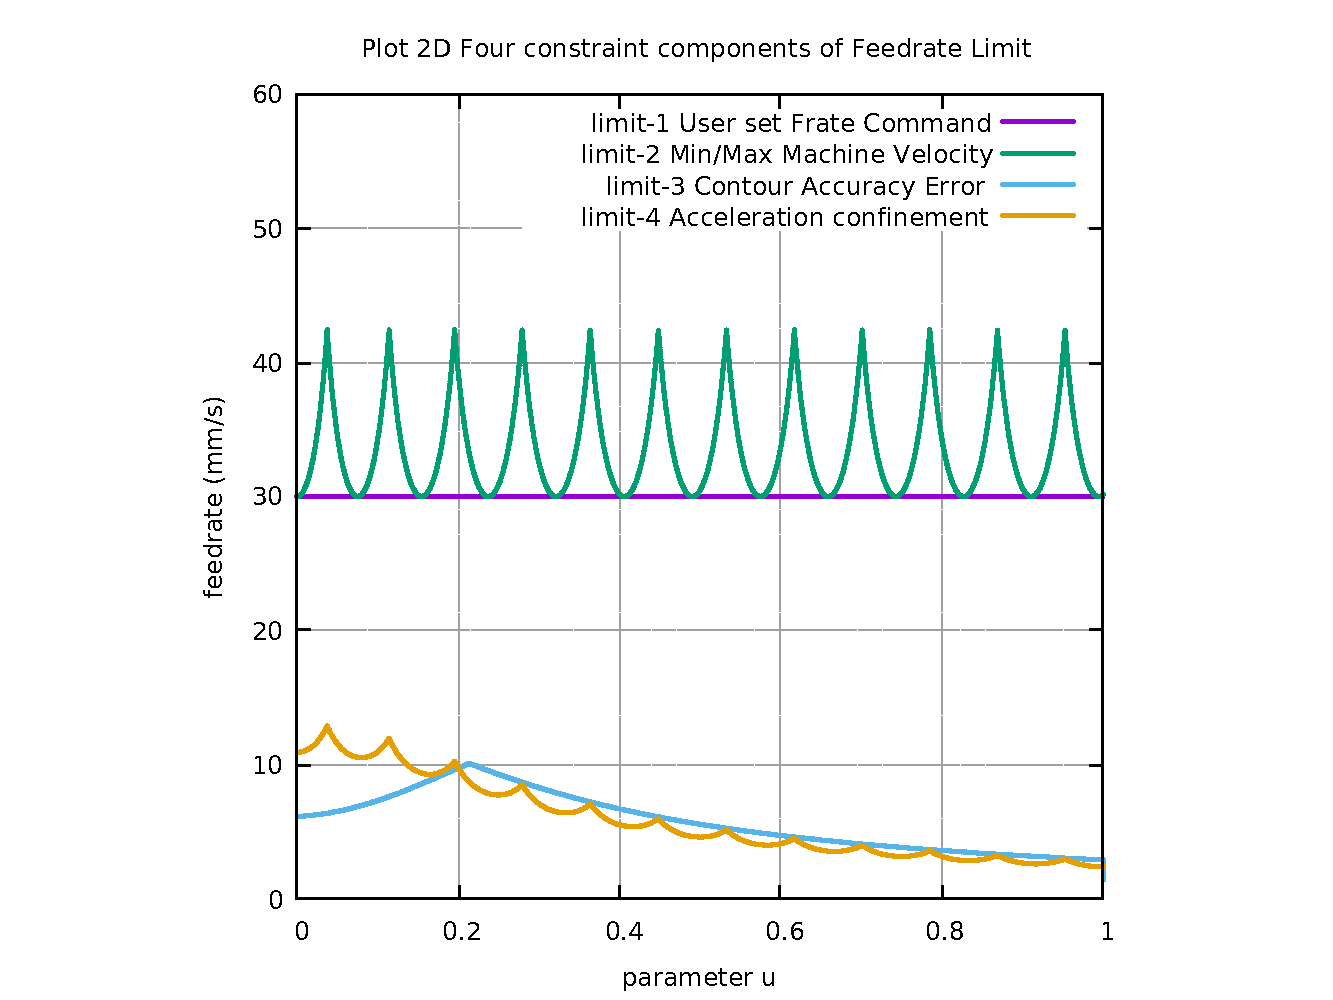
\includegraphics[width=1.00\textwidth]{Chap4/appendix/app-Snailshell/plots/33-img-Snailshell-FC30-Four-Components-FeedrateLimit.pdf}
\end{figure}


\begin{figure}
	\caption     {Snailshell FC40 Four Components FeedrateLimit}
	\label{34-img-Snailshell-FC40-Four-Components-FeedrateLimit.pdf}
	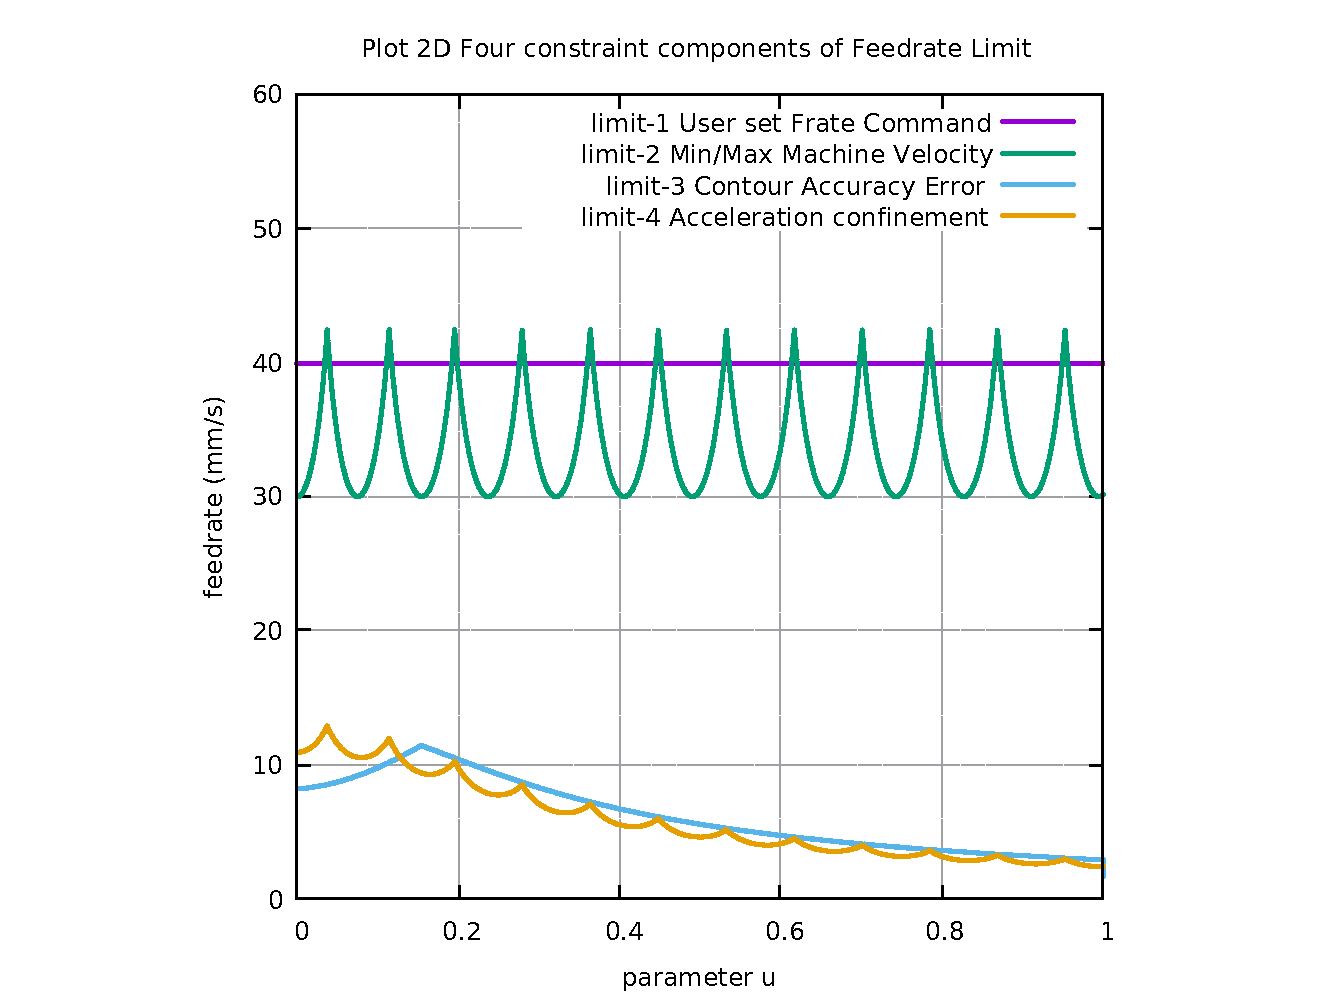
\includegraphics[width=1.00\textwidth]{Chap4/appendix/app-Snailshell/plots/34-img-Snailshell-FC40-Four-Components-FeedrateLimit.pdf}
\end{figure}


%% =======================================
\clearpage
\pagebreak

\begin{figure}
	\centering
	\caption     {Snailshell Histogram Points FC10 FC20 FC30 FC40}
	\label{35-img-Snailshell-Histogram-Points-FC10-FC20-FC30-FC40.pdf}
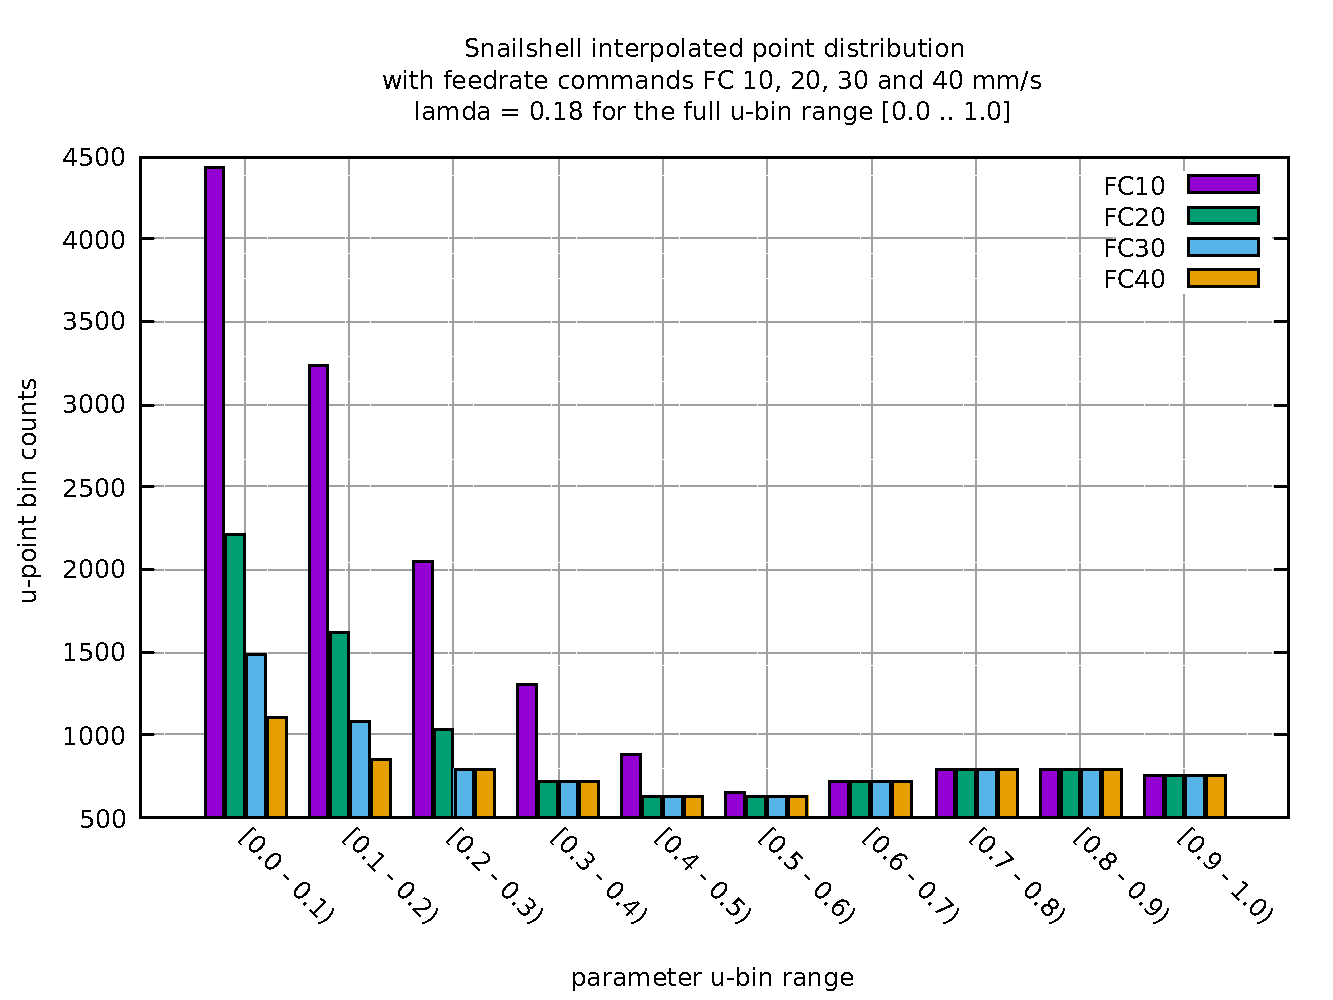
\includegraphics[width=1.00\textwidth]{Chap4/appendix/app-Snailshell/plots/35-img-Snailshell-Histogram-Points-FC10-FC20-FC30-FC40.pdf} 
\end{figure}


\begin{table}[ht]
%% \begin{center}
\caption    {Snailshell Table distribution of interpolated points}
\label  {tab-Snailshell Table distribution of interpolated points}
	
%% IMPORTANT TO SCALEBOX BELOW
\scalebox{0.80}{
		
%% START COPY AND PASTE BELOW HERE
%% FROM \begin{tabular} UNTIL \end{tabular)
%% Note: adjust last p{} to get line width correct
		
\begin{tabular}{ p{4.5cm} p{1.5cm} p{1.5cm} p{1.5cm} p{7.50cm} }
\hline
	&		&		&		&		\\
BINS	&	FC10	&	FC20	&	FC30	&	FC40	\\
&		&		&		&		\\
0.0 - 0.1	&	4435	&	2218	&	1479	&	1109	\\
0.1 - 0.2	&	3237	&	1619	&	1080	&	849	\\
0.2 - 0.3	&	2054	&	1028	&	796	&	793	\\
0.3 - 0.4	&	1312	&	714	&	711	&	711	\\
0.4 - 0.5	&	881	&	629	&	629	&	629	\\
0.5 - 0.6	&	657	&	628	&	629	&	628	\\
0.6 - 0.7	&	710	&	711	&	710	&	711	\\
0.7 - 0.8	&	794	&	794	&	794	&	794	\\
0.8 - 0.9	&	791	&	791	&	792	&	792	\\
0.9 - 1.0	&	750	&	751	&	750	&	750	\\
&		&		&		&		\\
Tot Counts	&	15621	&	9883	&	8370	&	7766	\\
&		&		&		&		\\
\hline	
\end{tabular}
		
%% END COPY AND PASTE ABOVE HERE
		
}   %% IMPORTANT FOR SCALEBOX CLOSING
	
\end{table}
%% \end{landscape}

%% Snailshell SUMMARY TABLE
%% ========================================================
\clearpage
\pagebreak
\begin{landscape}
	
\begin{table}[ht]
%% \begin{center}
\caption       {Snailshell Table FC10-20-30-40 Run Performance data}
\label{tab-app4-Snailshell-Table-FC10-20-30-40-Run-Performance-data}
		
% IMPORTANT TO SCALEBOX BELOW
\scalebox{0.90}{
			
%% START COPY AND PASTE BELOW HERE
%% FROM \begin{tabular} UNTIL \end{tabular)
			
			
\begin{tabular}{ p{0.2cm} p{8.80cm} p{4.00cm} p{4.0cm} p{4.00cm} p{4.0cm}}
	\hline
	&		&		&		&		&		\\
	1	&	Curve Type	&	SNAILSHELL	&	SNAILSHELL	&	SNAILSHELL	&	SNAILSHELL	\\
	2	&	User Feedrate Command FC(mm/s)                   	&	FC10	&	FC20	&	FC30	&	FC40	\\
	3	&	User Lamda Acceleration Safety Factor	&	0.18	&	0.18	&	0.18	&	0.18	\\
	&		&		&		&		&		\\
	4	&	Total Iterpolated Points (TIP)	&	15621	&	9883	&	8370	&	7766	\\
	5	&	Total Sum-Chord-Error (SCE) (mm)	&	5.115139395656E-03	&	6.269762299809E-03	&	6.764496555494E-03	&	7.045829082053E-03	\\
	6	&	Ratio 1 = (SCE/TIP) = Chord-Error/Point	&	3.274737129101E-07	&	6.344628921078E-07	&	8.082801476275E-07	&	9.073830112110E-07	\\
	&		&		&		&		&		\\
	7	&	Total Sum-Arc-Length (SAL) (mm)	&	1.385725614787E+02	&	1.385823558880E+02	&	1.385855208343E+02	&	1.385878579474E+02	\\
	8	&	Total Sum-Chord-Length (SCL) (mm)	&	1.385595406106E+02	&	1.385613905727E+02	&	1.385601641834E+02	&	1.385598862029E+02	\\
	9	&	Difference = (SAL – SCL) (mm)	&	1.302086811782E-02	&	2.096531529295E-02	&	2.535665098060E-02	&	2.797174444973E-02	\\
	10	&	Percentage Difference = (SAL – SCL)/SAL	&	9.396425943836E-03	&	1.512841599395E-02	&	1.829675338949E-02	&	2.018340196899E-02	\\
	&		&		&		&		&		\\
	11	&	Ratio 2 = (SCE/SCL) = Chord Error/Chord-Length	&	3.691654413053E-05	&	4.524898511695E-05	&	4.881992306637E-05	&	5.085042486059E-05	\\
	&		&		&		&		&		\\
	12	&	Total Sum-Arc-Theta (SAT) (rad)	&	1.894562150080E+01	&	1.894533592343E+01	&	1.894325318416E+01	&	1.894232057270E+01	\\
	13	&	Total Sum-Arc-Area (SAA) (mm2)	&	1.070830851582E-04	&	3.068808285119E-04	&	5.164360050036E-04	&	7.283849492346E-04	\\
	&		&		&		&		&		\\
	14	&	Ratio 3 = (SAA/SCL) = Arc-Area/Chord-Length	&	3.691654413053E-05	&	4.524898511695E-05	&	4.881992306637E-05	&	5.085042486059E-05	\\
	&		&		&		&		&		\\
	15	&	Average-Chord-Error (ACE) (mm)	&	3.274737129101E-07	&	6.344628921078E-07	&	8.082801476275E-07	&	9.073830112110E-07	\\
	16	&	Average-Arc-Length (AAL) (mm)	&	8.871482809134E-03	&	1.402371543089E-02	&	1.655938831812E-02	&	1.784776019928E-02	\\
	17	&	Average-Chord-Length (ACL) (mm)	&	8.870649206822E-03	&	1.402159386488E-02	&	1.655635848768E-02	&	1.784415791409E-02	\\
	18	&	Average-Arc-Theta (AAT) (rad)	&	1.212907906581E-03	&	1.917156033539E-03	&	2.263502591010E-03	&	2.439448882512E-03	\\
	19	&	Average-Arc-Area (AAA) (mm2)	&	6.855511213715E-09	&	3.105452626107E-08	&	6.170820946393E-08	&	9.380359938629E-08	\\
	&		&		&		&		&		\\
	20	&	Algorithm actual runtime on computer (ART) (s) 	&	17.308275283	&	24.17500989	&	29.295160546	&	32.06253681	\\
	&		&		&		&		&		\\
	\hline
	
\end{tabular}
			
%% END COPY AND PASTE		
}   %% IMPORTANT FOR SCALEBOX CLOSING
		
\end{table}
\end{landscape}

%% =======================================
\clearpage
\pagebreak
